\graphicspath{{./chapters/chapter3/}}
\chapter{ }

\allowdisplaybreaks[1]

% \section{Basic Notation}
% \label{chap3-sec:notation_table}
% Table~\ref{chap3-tab:notations} shows the basic notation used in this paper. 

\section{Experiments of the Clustering Coefficient}
\label{chap3-sec:cluster}
In Section~\ref{chap3-sec:experiments}, we showed that our triangle counting algorithm \AlgWSTriVR{} accurately estimates the triangle count within one round.
We also show that we can accurately estimate the clustering coefficient within one round by using \AlgWSTriVR{}.

We calculated the clustering coefficient as follows.
We used \AlgWSTriVR{} ($c=1$) for triangle counting and
the one-round local algorithm in \cite{Imola_USENIX21} with edge clipping \cite{Imola_USENIX22}
% the one-round algorithm in \cite{Imola_USENIX22} (a modification of the algorithm in \cite{Imola_USENIX21} using edge clipping)
for 2-star counting.
% Specifically, for 2-stars,
The 2-star algorithm works as follows.
First, each user $v_i$ adds the Laplacian noise $\Lap(\frac{1}{\epsilon_1})$ and a non-negative constant $\eta \in \nnreals$ to her degree $d_i$ to obtain a noisy degree $\td_i = d_i + \Lap(\frac{1}{\epsilon_1}) + \eta$ with $\epsilon_1$-edge LDP.
% Because the sensitivity of $d_i$ is $1$, the noisy degree $\td_i$ provides $\epsilon_1$-edge LDP.
If $\td_i < d_i$, then $v_i$ randomly removes $d_i - \lfloor \td_i \rfloor$ neighbors from her neighbor list.
This is called edge clipping in \cite{Imola_USENIX22}.
Then, $v_i$ calculates the number $r_i \in \nnints$ of 2-stars of which she is a center.
User $v_i$ adds $\Lap(\frac{\td_i}{\epsilon_2})$ to $r_i$ to obtain a noisy 2-star count $\tilde{r}_i = r_i + \Lap(\frac{\td_i}{\epsilon_2})$.
Because the sensitivity of the $k$-star count is $\binom{\td_i}{k-1}$, the noisy 2-star count $\tilde{r}_i$ provides $\epsilon_2$-edge LDP.
User $v_i$ sends the noisy degree $\td_i$ and the noisy 2-star count $\tilde{r}_i$ to the data collector.
Finally, the data collector estimates the 2-star count as $\sum_{i=1}^n \tilde{r}_i$.
By composition, this algorithm provides $(\epsilon_1 + \epsilon_2)$-edge LDP.
As with \cite{Imola_USENIX22}, we set $\eta = 150$ and divided the total privacy budget $\epsilon$ as $\epsilon_1 = \frac{\epsilon}{10}$ and $\epsilon_1 = \frac{9\epsilon}{10}$.

Let $\hf^\triangle(G)$ be the estimate of the triangle count by \AlgWSTriVR{} and $\hf^{2*}(G)$ be the estimate of the 2-star count by the above algorithm.
Then we estimated the clustering coefficient as $\frac{3 \hf^\triangle(G)}{\hf^{2*}(G)}$.

Figure~\ref{chap3-fig:res6_clst} shows the relative errors of the triangle count, 2-star count, and clustering coefficient in \Gplus{} and \IMDB{}.
We observe that the relative error of the clustering coefficient is almost the same as that of the triangle count.
This is because the 2-star algorithm is very accurate, as shown in Figure~\ref{chap3-fig:res6_clst}.
2-stars are much easier to count than triangles in the local model, as each user can count her 2-stars.
As a result, the error in the clustering coefficient is mainly caused by the error in $\hf^\triangle(G)$, which explains the results in Figure~\ref{chap3-fig:res6_clst}.

In Figure~\ref{chap3-fig:res6_clst}, we use the privacy budget $\epsilon$ for both $\hf^\triangle(G)$ and $\hf^{2*}(G)$.
%. Thus, we need $2\epsilon$ in element DP
% to calculate the clustering coefficient.
In this case, we need $2\epsilon$ to calculate the clustering coefficient.
% in Figure~\ref{chap3-fig:res6_clst}.
However, as shown in Figure~\ref{chap3-fig:res6_clst}, we can accurately estimate the 2-star count with a very small $\epsilon$; e.g., the relative error is around $10^{-2}$ when $\epsilon=0.1$.
Therefore, we can accurately calculate the clustering coefficient
% in the same way as triangles
with a very small additional budget
% almost the same privacy budget as triangles
by using such a small $\epsilon$ for 2-stars.

In summary, our triangle algorithm \AlgWSTriVR{} is useful for accurately calculating the clustering coefficient within one round.

% \begin{table}[t]
% \caption{Basic notation in this paper.}
% 
% \centering
% \hbox to\hsize{\hfil
% \begin{tabular}{l|l}
% \hline
% Symbol		&	Description\\
% \hline
% % $I_{-(i,j)}$    &   Set of user indices other than $i$ and $j$ ($[n]\setminus\{i,j\}$).\\
% $G=(V,E)$   &	    Undirected social graph.\\
% $n$         &	    Number of nodes (users).\\
% $v_i$       &       $i$-th user in $V$, i.e., $V=\{v_1,\ldots,v_n\}$.\\
% % $I_{-(i,j)}$    &   Set of user indices other than $i$ and $j$ ($[n]\setminus\{i,j\}$).\\
% $I_{-(i,j)}$    &   $=[n]\setminus\{i,j\}$.\\
% $d_i$   &       Degree of $v_i$.\\
% $d_{avg}$   &       Average degree in $G$.\\
% $d_{max}$   &       Maximum degree in $G$.\\
% $\calG$     &       Set of possible graphs with $n$ nodes.\\
% $f^\triangle(G)$   &  Triangle count in graph $G$.\\
% $f^\square(G)$   &  4-cycle count in graph $G$.\\
% % $\hf^\triangle(G)$   &  Estimate of the triangle count in graph $G$.\\
% $\bmA=(a_{i,j})$	    &		Adjacency matrix.\\
% % $a_{i,j}$	&		Edge indicator between $v_i$ and $v_j$.\\
% $\bma_i$	&		Neighbor list of $v_i$, i.e., the $i$-th row of $\bmA$.\\
% % $\calR_i$     &       Local randomizer of $v_i$.\\
% \hline
% \end{tabular}
% \hfil}
% \label{chap3-tab:notations}
% \end{table}

\begin{figure}[t]
  \centering
  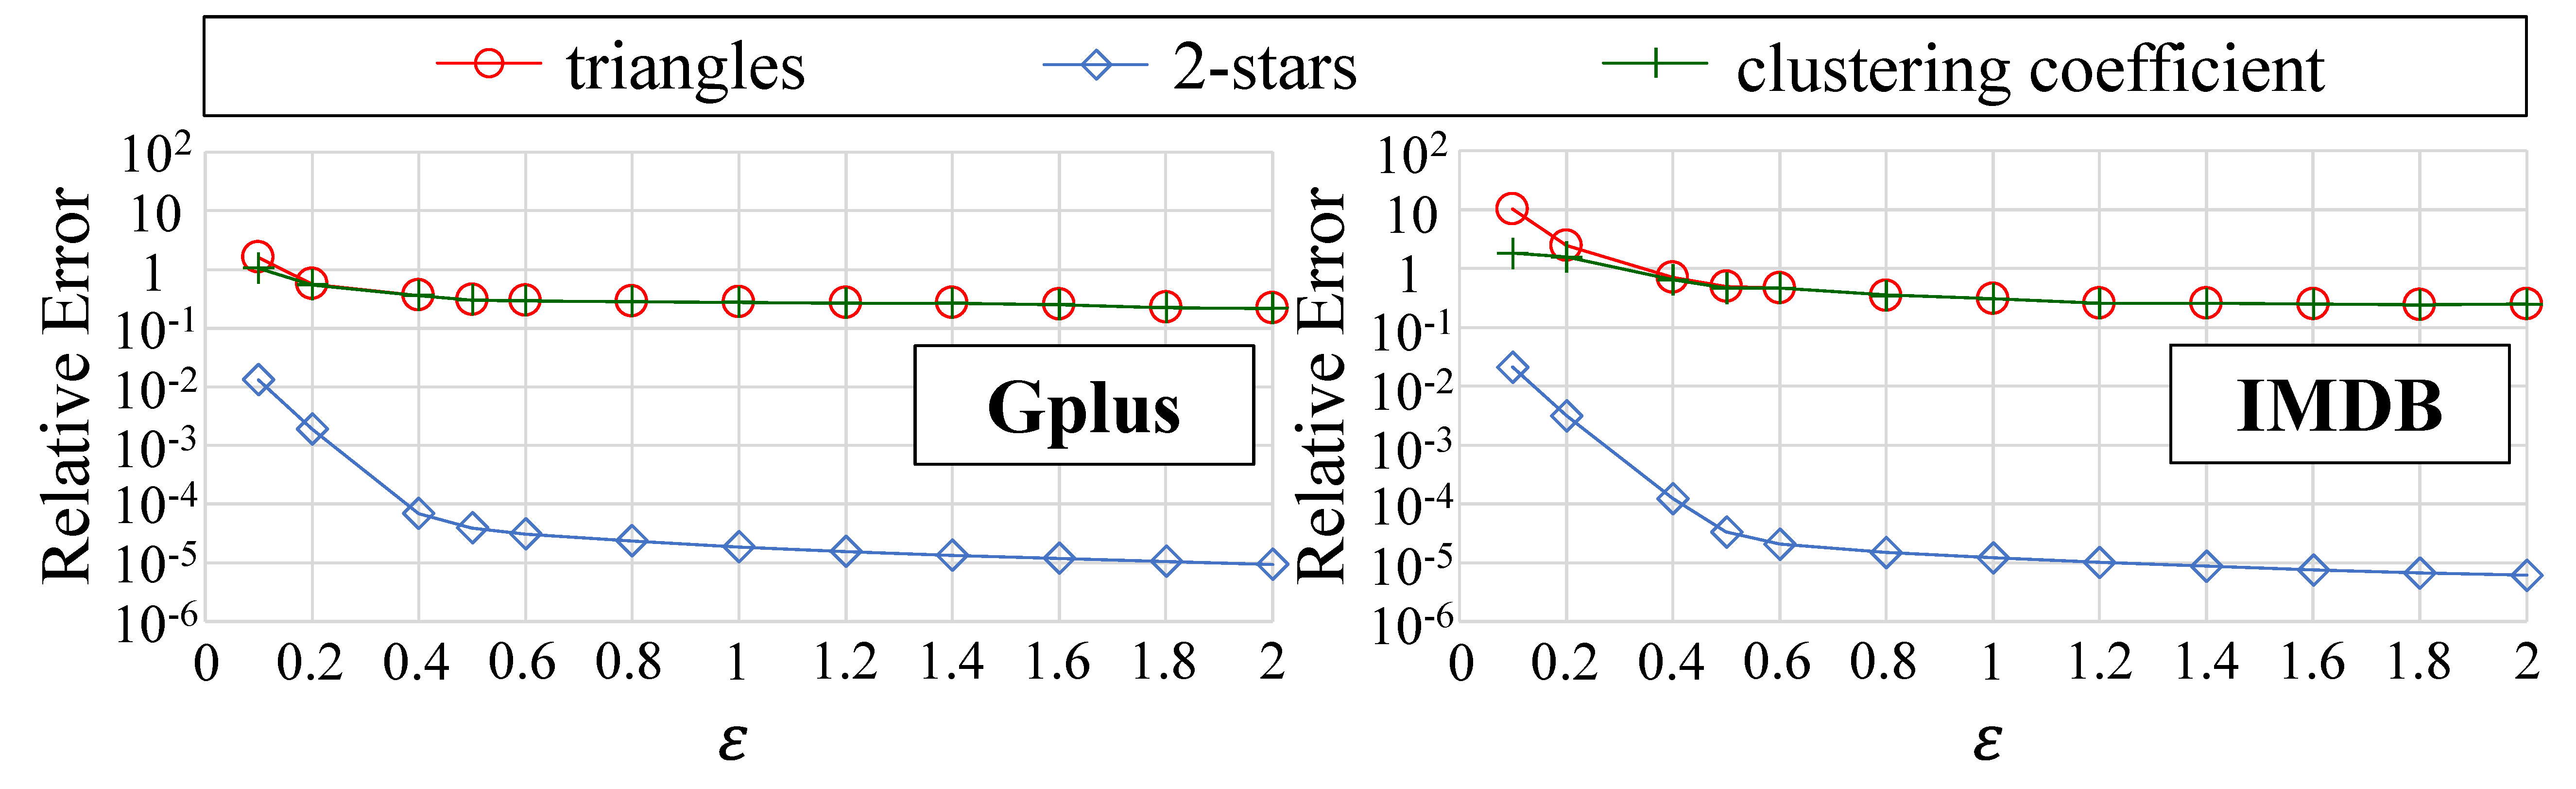
\includegraphics[width=0.99\linewidth]{fig/res6_clst.pdf}
  
  \caption[Relative errors of the triangle count, 2-star count, and clustering coefficient when \AlgWSTriVR{} and the one-round local 2-star algorithm with edge clipping are used.]
{Relative errors of the triangle count, 2-star count, and clustering coefficient when \AlgWSTriVR{} and the one-round local 2-star algorithm in \cite{Imola_USENIX21} with edge clipping are used ($n=107614$ in \Gplus{}, $n=896308$ in \IMDB{}, $c=1$).
  }
  \label{chap3-fig:res6_clst}
\end{figure}

% \smallskip
% \noindent{\textbf{Comparison with Two-Round Local Algorithms.}}~~
\section{Comparison with Two-Round Local Algorithms}
\label{chap3-sec:two-round}
In this work, we focus on one-round algorithms because multi-rounds algorithms require a lot of user effort and synchronization.
However, it is interesting to see how our one-round algorithms compare with the existing two-round local algorithms \cite{Imola_USENIX21,Imola_USENIX22} in terms of accuracy, as the existing two-round algorithms provide high accuracy.
%small estimation errors.
Since they focus on triangle counting, we focus on this task.
% Here, we focus on triangle counting because the existing two-round algorithms focus on this task.
% We also compared our triangle algorithms with the existing two-round local algorithms \cite{Imola_USENIX21,Imola_USENIX22}.

We evaluate the two-round local algorithm in \cite{Imola_USENIX22} because it outperforms \cite{Imola_USENIX21} in terms of both the accuracy and communication efficiency.
The algorithm in \cite{Imola_USENIX22} works as follows.
At the first round, each user $v_i$ obfuscates bits $a_{i,1}, \ldots, a_{i,i-1}$ for smaller user IDs in her neighbor list $\bma_i$ (i.e., lower triangular part of $\bmA$) by the ARR and sends the noisy neighbor list to the data collector.
The data collector constructs a noisy graph $G'=(V,E')$ from the noisy neighbor lists.
At the second round, each user $v_i$ downloads some noisy edges $(v_j,v_k) \in E'$
% between other users
from the data collector and counts noisy triangles $(v_i, v_j, v_k)$ so that
% Note that
only one edge $(v_j, v_k)$ is noisy.
% in each noisy triangle.
User $v_i$ adds the Laplacian noise to the noisy triangle count and sends it to the data collector.
Finally, the data collector calculates an unbiased estimate of the triangle count.
This algorithm provides $\epsilon$-edge LDP.
The authors in \cite{Imola_USENIX22} propose some strategies to select noisy edges to download at the second round.
We use a strategy to download noisy edges $(v_j,v_k) \in E'$ such that a noisy edge is connected from $v_k$ to $v_i$ (i.e., $(v_i,v_k) \in E'$) because it provides the best performance.

The algorithm in \cite{Imola_USENIX22} controls the trade-off between the accuracy and the download cost (i.e., the size of noisy edges) at the second round by changing the sampling probability $p_0$ in the ARR.
It is shown in \cite{Imola_USENIX22} that
when $p_0 = 1$, the MSE is $O(n d_{max}^3)$ and the download cost of each user is $\frac{(n-1)(n-2)}{2}$ bits.
% $n^2 \log n$.
In contrast,
when $p_0 = O(n^{-1/2})$, the MSE is $O(n^2 d_{max}^3)$ and the download cost is $O(n \log n)$.
% We evaluated both the efficient and inefficient settings.
We evaluated these two settings.
% For the efficient setting,
For the latter setting,
% we set $p_0$ so that $p_0 q = \frac{1}{n}$, where $q=\frac{e^\epsilon}{e^\epsilon+1}$.
% In this case, the download cost is $n \log n$ bits.
we set $p_0 = \frac{1}{q \sqrt{n}}$ where $q=\frac{e^\epsilon}{e^\epsilon+1}$ so that the download cost is $n \log n$ bits.
We denote the two-round algorithm with $p_0=1$ and $\frac{1}{q \sqrt{n}}$ by \AlgTwoRL{} and \AlgTwoRS{}, respectively.
% (\AlgTwoRL{} and \AlgTwoRS{} need large and small download costs, respectively).
\AlgTwoRL{} requires a larger download cost.

\begin{figure}[t]
  \centering
  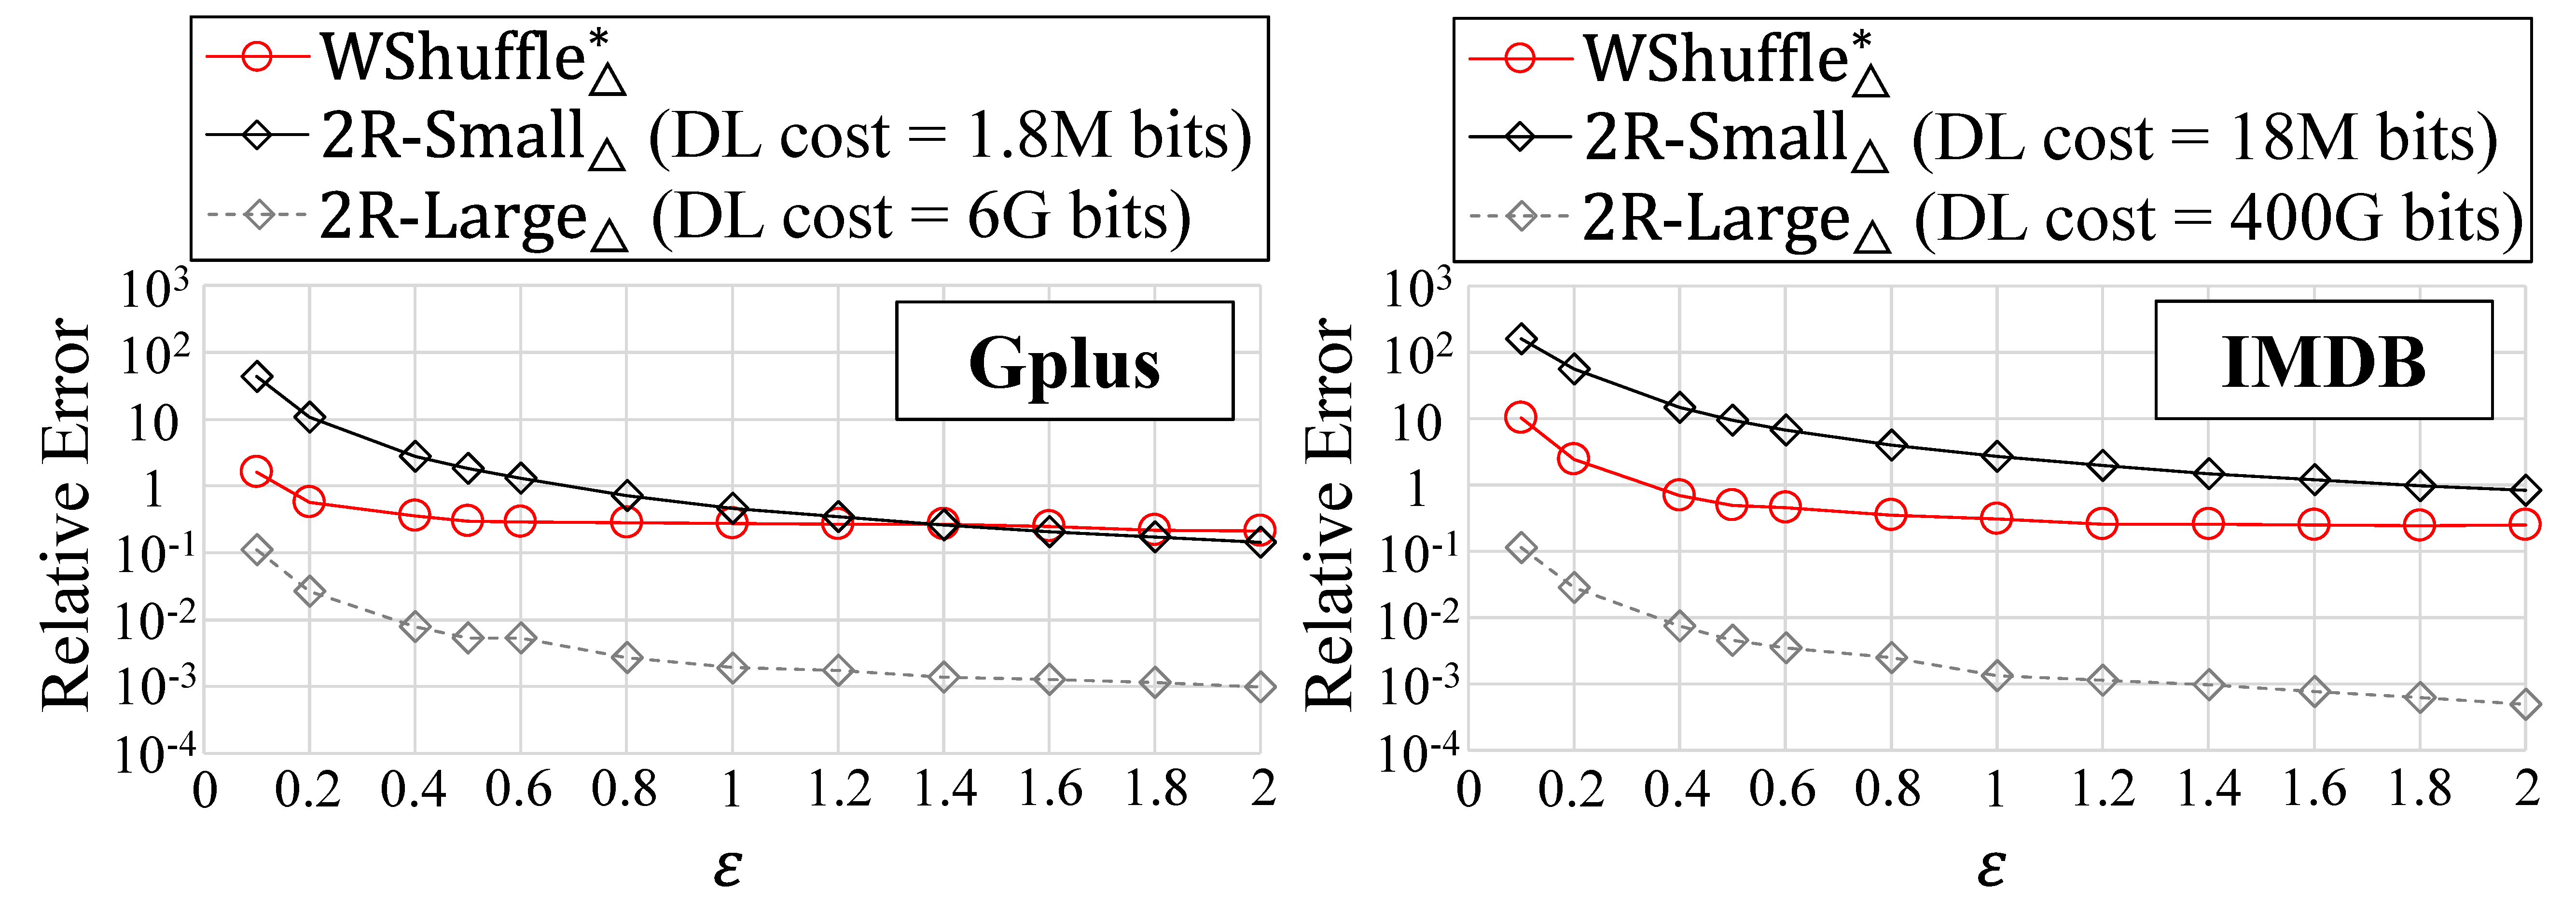
\includegraphics[width=0.99\linewidth]{fig/res3_2rounds.pdf}
  
  \caption[Comparison with the two-round local algorithm in~\cite{Imola_USENIX22}.]{Comparison with the two-round local algorithm in \cite{Imola_USENIX22}.
  The download costs of \AlgTwoRS{} and \AlgTwoRL{} are $n \log n$ and $\frac{(n-1)(n-2)}{2}$ bits, respectively
  ($n=107614$ in \Gplus{}, $n=896308$ in \IMDB{}, $c=1$).
  }
  \label{chap3-fig:res3_2rounds}
\end{figure}

Figure~\ref{chap3-fig:res3_2rounds} shows the results.
We observe that our \AlgWSTriVR{} is outperformed by \AlgTwoRL{}.
This is expected, as \AlgWSTriVR{} and \AlgTwoRL{} provide the MSE of $O(n^2)$ and $O(n)$, respectively (when we ignore $d_{max}$).
However, \AlgTwoRL{} is impractical because it requires a too large download cost: 6G and 400G bits per user in \Gplus{} and \IMDB{}, respectively.
\AlgTwoRS{} is much more efficient (1.8M and 18M bits in \Gplus{} and \IMDB{}, respectively), and our \AlgWSTriVR{} is comparable to or outperforms \AlgTwoRS{}\footnote{As with \AlgARRTri{}, \AlgTwoRL{} and \AlgTwoRS{} provide $\epsilon$-edge DP (rather than $2\epsilon$-edge DP) because it uses only the lower-triangular part of $\bmA$.
However, our conclusion is the same even if we double $\epsilon$ for only \AlgWSTriVR{}.}.
This is also consistent with the theoretical results because both \AlgWSTriVR{} and \AlgTwoRS{} provide the MSE of $O(n^2)$.

In summary, our \AlgWSTriVR{} is comparable to the two-round local algorithm in \cite{Imola_USENIX22} (\AlgTwoRS{}), which requires a lot of user effort and synchronization, in terms of accuracy.

\section{Comparison between the Numerical Bound and the Closed-form Bound}
\label{chap3-sec:numerical_closed}
In Section~\ref{chap3-sec:experiments}, we used the numerical upper bound in \cite{Feldman_FOCS21} for calculating $\epsilon$ in the shuffle model.
Here, we compare the numerical bound with the closed-form bound in Theorem~\ref{chap3-thm:shuffle}.

\begin{figure}[t]
  \centering
  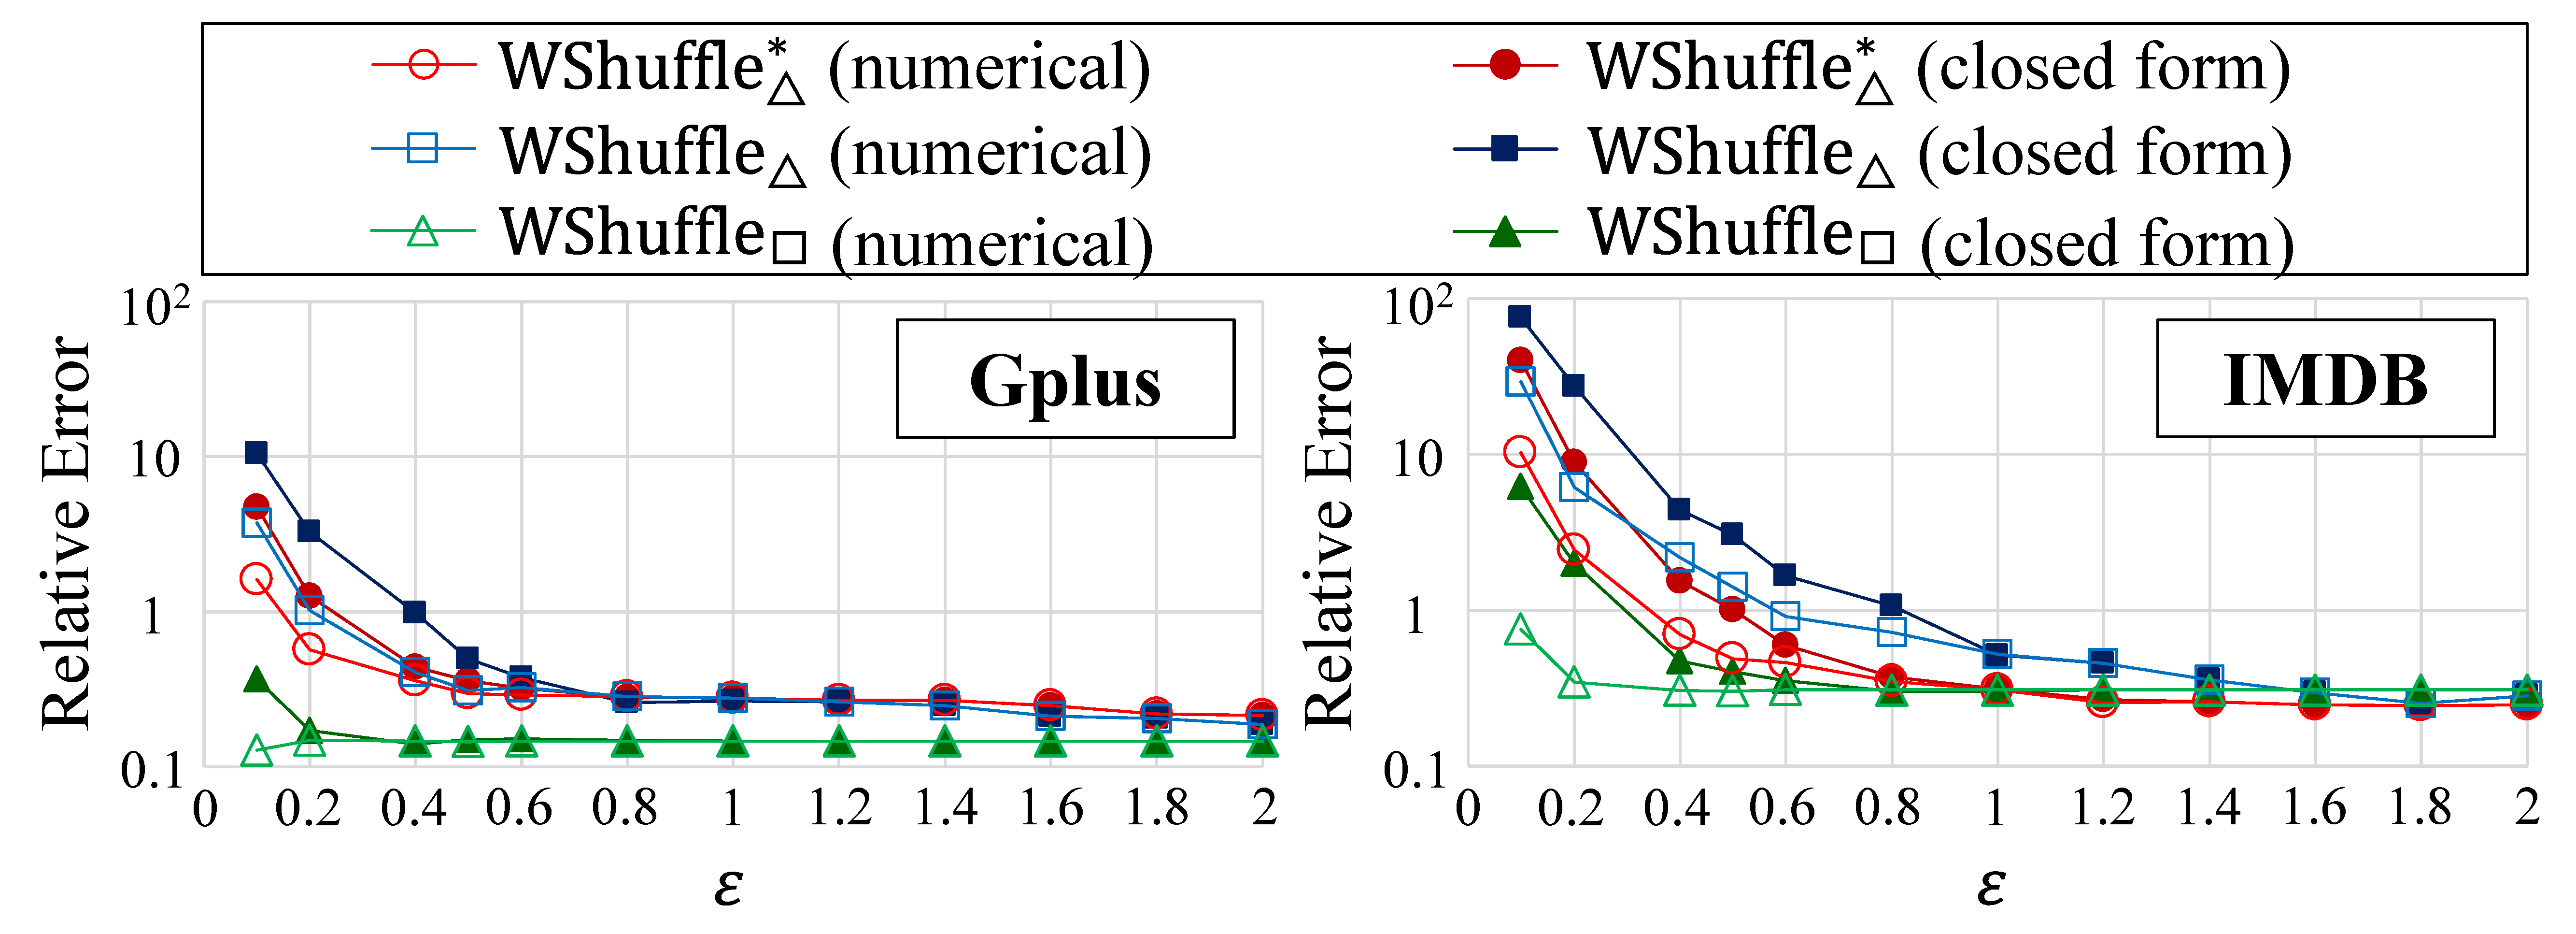
\includegraphics[width=0.99\linewidth]{fig/res5_closed.pdf}
  
  \caption[Numerical bound vs. closed-form bound.]{Numerical bound vs. closed-form bound ($n=107614$ in \Gplus{}, $n=896308$ in \IMDB{}, $c=1$).
  }
  \label{chap3-fig:res5_closed}
\end{figure}

Figure~\ref{chap3-fig:res5_closed} shows the results for \AlgWSTriVR{}, \AlgWSTri{}, and \AlgWSCyc{}.
We observe that the numerical bound provides a smaller relative error than the closed-form bound when $\epsilon$ is small.
However, when $\epsilon \geq 1$, the relative error is almost the same between the numerical bound and the closed-form bound.
This is because when $\epsilon \geq 1$, the corresponding $\epsilon_L$ is close to the maximum value $\log (\frac{n}{16 \log (2/\delta)})$ ($=5.86$ in \Gplus{} and $7.98$ in \IMDB{}) in both cases.
Thus, for a large $\epsilon$, the closed-form bound is sufficient.
For a small $\epsilon$, the numerical bound is preferable.

\section{Experiments on the Barab\'{a}si-Albert Graphs}
\label{chap3-sec:BA-graph}
In Section~\ref{chap3-sec:experiments}, we used \Gplus{} and \IMDB{} as datasets.
We also evaluated our algorithms using synthetic datasets based on the BA (Barab\'{a}si-Albert) graph model \cite{NetworkScience}, which has a power-law degree distribution.
% \cite{NetworkScience,Hagberg_SciPy08},

The BA graph model generates a graph by adding new nodes one at a time.
Each new node has $m \in \nats$ new edges, and each new edge is randomly connected an existing node with probability proportional to its degree.
The average degree is almost $d_{avg} = 2m$, and most users' degrees are $m$.
We set $m=100$ or $200$ and used the NetworkX library \cite{Hagberg_SciPy08} (barabasi\_albert\_graph function) to generate a synthetic graph based on the BA model.
For the number $n$ of users, we set $n=107614$ (same as \Gplus{}) to compare the results between \Gplus{} and the BA graphs.
Table~\ref{chap3-tab:BA_graphs} shows some statistics of \Gplus{} and the BA graphs.
It is well known that the BA model has a low clustering coefficient \cite{Holme_PRE02}.
Thus, the BA graphs have much smaller triangles and 4-cycles than \Gplus{}.

\begin{table}[t]
  \caption[Statistics of \Gplus{} and the Barab\'{a}si-Albert graphs.]{Statistics of \Gplus{} and the BA graphs ($n=107614$).
  }
  
  \centering
  \begin{tabular}{|c|c|c|c|c|}
    \hline
    & $d_{avg}$ & $d_{max}$ & \#triangles & \#4-cycles\\ \hline
    \Gplus{} & $227.4$ & $20127$ & $1.07 \times 10^{9}$ & $1.42 \times 10^{12}$ \\ \hline
    BA ($m=100$) & $199.8$ & $5361$ & $1.56 \times 10^7$ & $5.31 \times 10^9$ \\ \hline
    BA ($m=200$) & $399.3$ & $7428$ & $9.86 \times 10^7$ & $6.21 \times 10^{10}$ \\ \hline
  \end{tabular}
  \label{chap3-tab:BA_graphs}
\end{table}

Figure~\ref{chap3-fig:res7_BA} shows the results in the BA graphs.
We observe that the relative error is smaller when $m=200$.
This is because the BA graph with $m=200$ includes larger numbers of true triangles and 4-cycles,
% the true triangle and 4-cycle counts are larger when $m=200$,
as shown in Table~\ref{chap3-tab:BA_graphs}.
In this case, the denominator in the relative error is larger, and consequently the relative error becomes smaller.
By Figures~\ref{chap3-fig:res1_eps} and \ref{chap3-fig:res7_BA}, the relative error in the BA graph with $m=100$ is larger than the relative error in \Gplus{}.
The reason for this is the same -- \Gplus{} includes larger numbers of triangles and 4-cycles, as shown in Table~\ref{chap3-tab:BA_graphs}.
% In other words, the relative error tends to be smaller in dense graphs.
These results show that the relative error tends to be smaller in a dense graph that includes a larger number of subgraphs.

\begin{figure}[t]
  \centering
  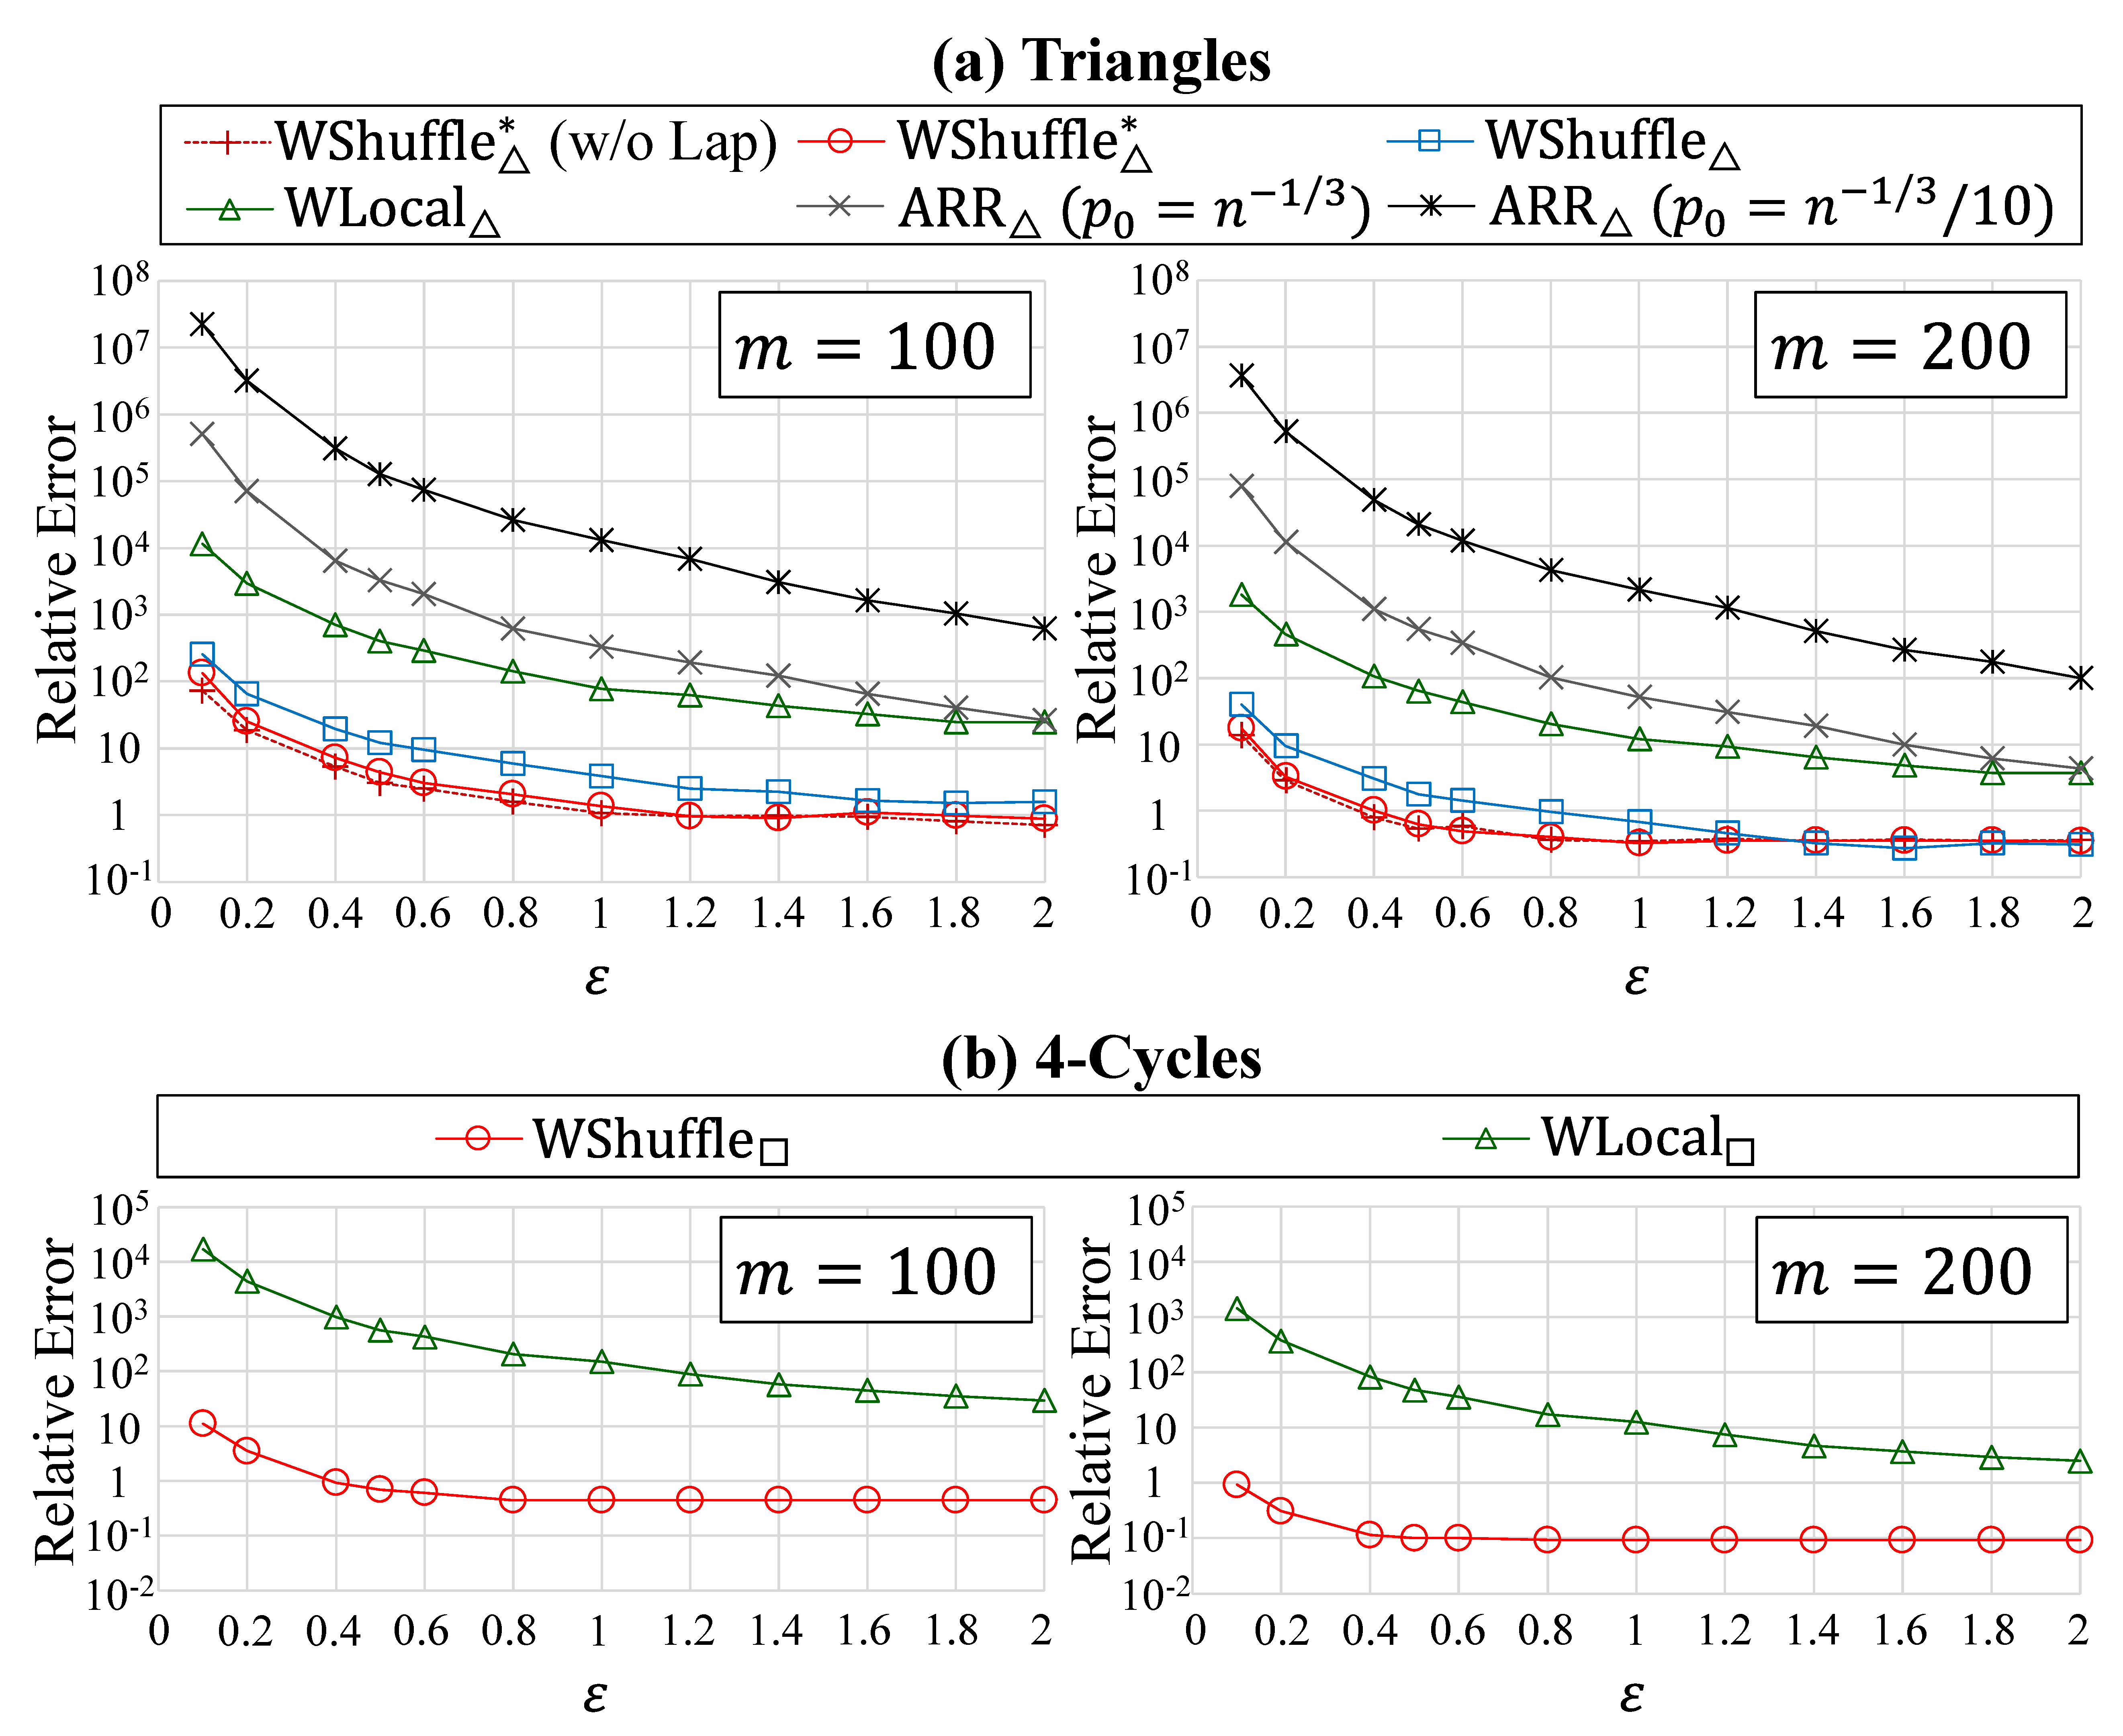
\includegraphics[width=0.99\linewidth]{fig/res7_BA.pdf}
  
  \caption[Relative error in the Barab\'{a}si-Albert graphs.]{Relative error in the BA graph data
  ($n=107614$, $c=1$).
  $p_0$ is the sampling probability in the ARR.
  }
  \label{chap3-fig:res7_BA}
%\end{figure}
\vspace{2mm}
%\begin{figure}[t]
  \centering
  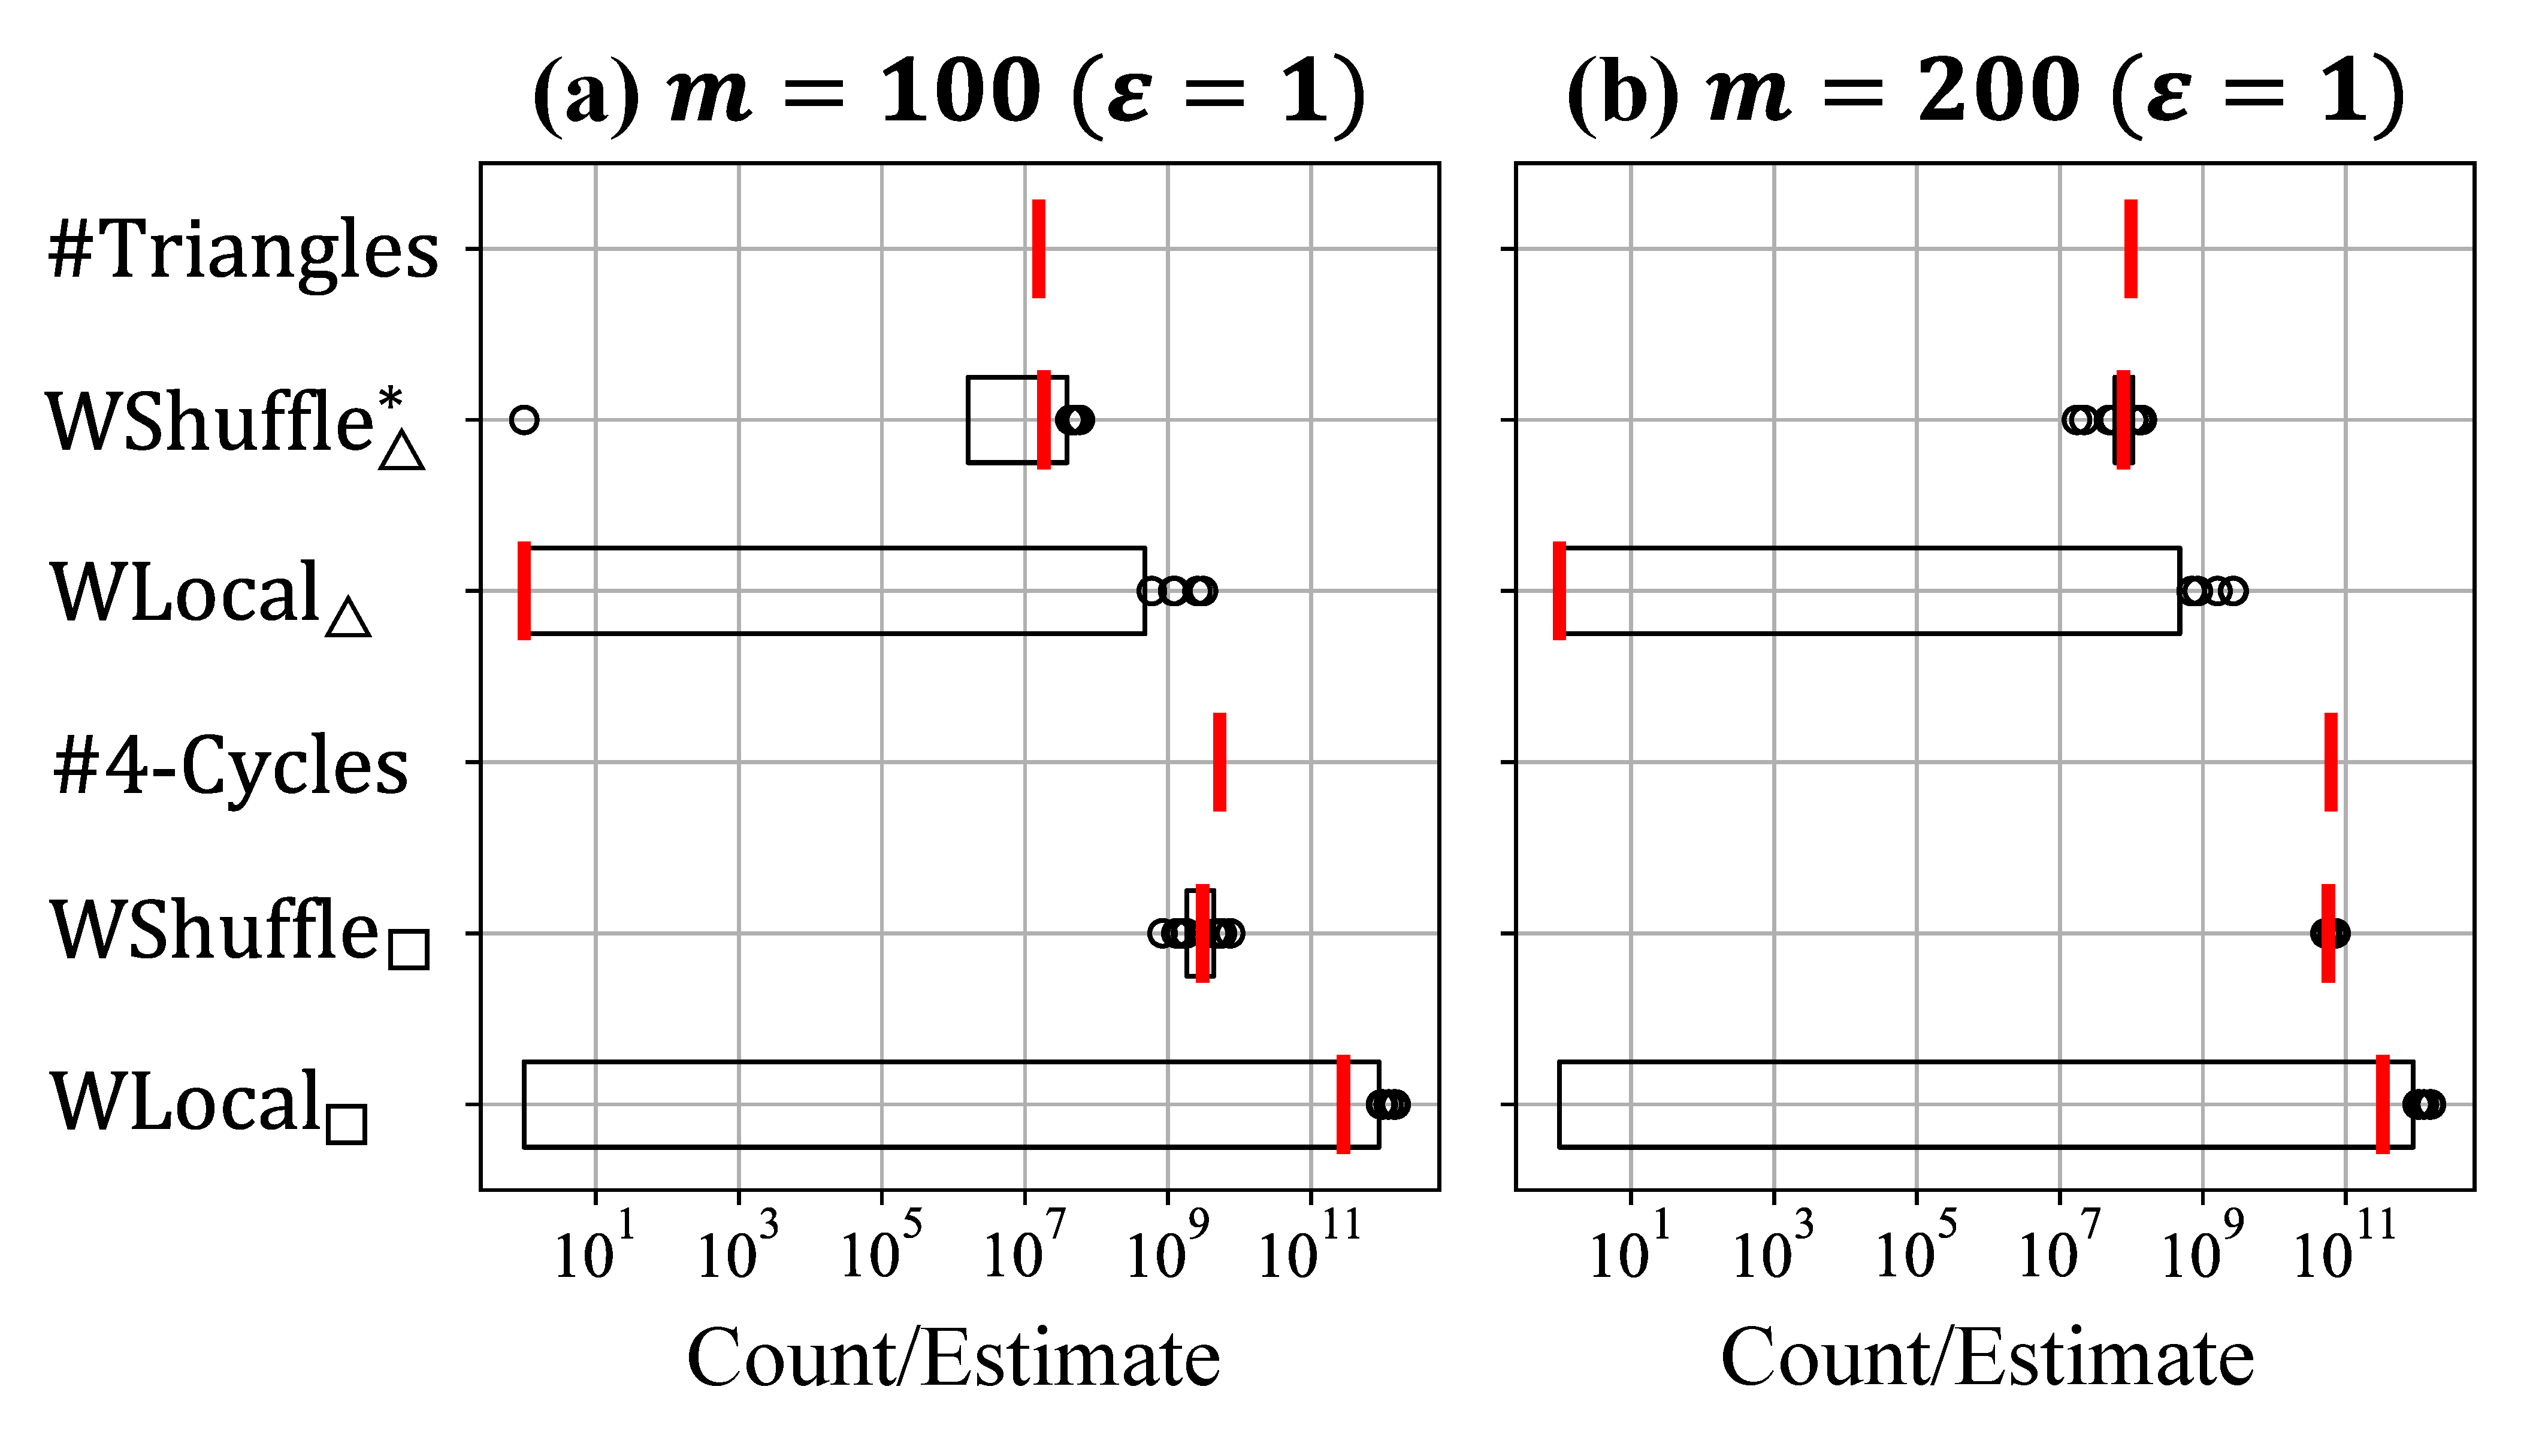
\includegraphics[width=0.8\linewidth]{fig/res7_BA_box.pdf}
  
  \caption[Box plots of counts/estimates in the Barab\'{a}si-Albert graphs.]{Box plots of counts/estimates in the BA graph data
  ($n=107614$, $c=1$).
  \#Triangles and \#4-Cycles represent the true triangle and 4-cycle counts, respectively.
  The box plot of each algorithm represents the median (red), lower/upper quartile, and outliers (circles) of $20$ estimates.
  The leftmost values are smaller than $1$.
  }
  \label{chap3-fig:res7_BA_box}
\end{figure}

Figures~\ref{chap3-fig:res7_BA} shows that when $\epsilon=1$, the relative errors of \AlgWSTriVR{} ($m=100$), \AlgWSCyc{} ($m=100$), \AlgWSTriVR{} ($m=200$), and \AlgWSCyc{} ($m=200$) are $1.36$, $0.447$, $0.323$, and $0.0928$, respectively.
Although the relative error of \AlgWSTriVR{} is about $1$ when $\epsilon=1$ and $m=100$, we argue that it is still useful for calculating a rough estimate of the triangle count.
To explain this, we show box plots of counts or estimates in the BA graphs in Figure~\ref{chap3-fig:res7_BA_box}.
This figure shows that the true triangle count is about $10^7$ and that \AlgWSTriVR{} ($m=100$) successfully calculates a rough estimate ($10^6 \sim 10^8$) in most cases ($15$ out of $20$ cases).
\AlgWSCyc{} ($m=100$), \AlgWSTriVR{} ($m=200$), and \AlgWSCyc{} ($m=200$) are much more accurate and successfully calculate an estimate in all cases.
In contrast, the local algorithms \AlgWLTri{} and \AlgWLCyc{} fail to calculate a rough estimate.

In summary, our shuffle algorithms significantly outperform the local algorithms and calculate a (rough) estimate of the triangle/4-cycle count with a reasonable privacy budget (e.g., $\epsilon=1$) in the BA graph data.

\section{Experiments on the Bipartite Graphs}
\label{chap3-sec:bipartite}
As described in Section~\ref{chap3-sec:intro}, the 4-cycle count is useful for measuring the clustering tendency in a bipartite graph where no triangles appear.
Therefore, we also evaluated our 4-cycle counting algorithms using bipartite graphs generated from \Gplus{} and \IMDB{}.

Specifically, for each dataset, we randomly divided all users into two groups with equal number of users.
The number of users in each group is $53807$ in \Gplus{} and $448154$ in \IMDB{}.
Then, we constructed a bipartite graph by removing edges within each group.
We refer to the bipartite versions of \Gplus{} and \IMDB{} as the \textit{bipartite \Gplus{}} and \textit{bipartite \IMDB{}}, respectively.
Using these datasets, we evaluated the relative errors of \AlgWSCyc{} and \AlgWLCyc{}.
Note that we did not evaluate the triangle counting algorithms, because there are no triangles in these graphs.

% \begin{table}[t]
%   \caption{4-cycle count in \Gplus{}, \IMDB{}, and the corresponding bipartite graphs (B: bipartite graph).
%   }
%   
%   \centering
%   \begin{tabular}{|c|c|c|c|}
%     \hline
%     \Gplus{} & \IMDB{} & \Gplus{} (B) & \IMDB{} (B)\\ \hline
%     $1.42 \times 10^{12}$ & $2.37 \times 10^{12}$ & $1.77 \times 10^{11}$ & $2.96 \times 10^{11}$ \\ \hline
%   \end{tabular}
%   \label{chap3-tab:BA_graphs}
% \end{table}

\begin{figure}[t]
  \centering
  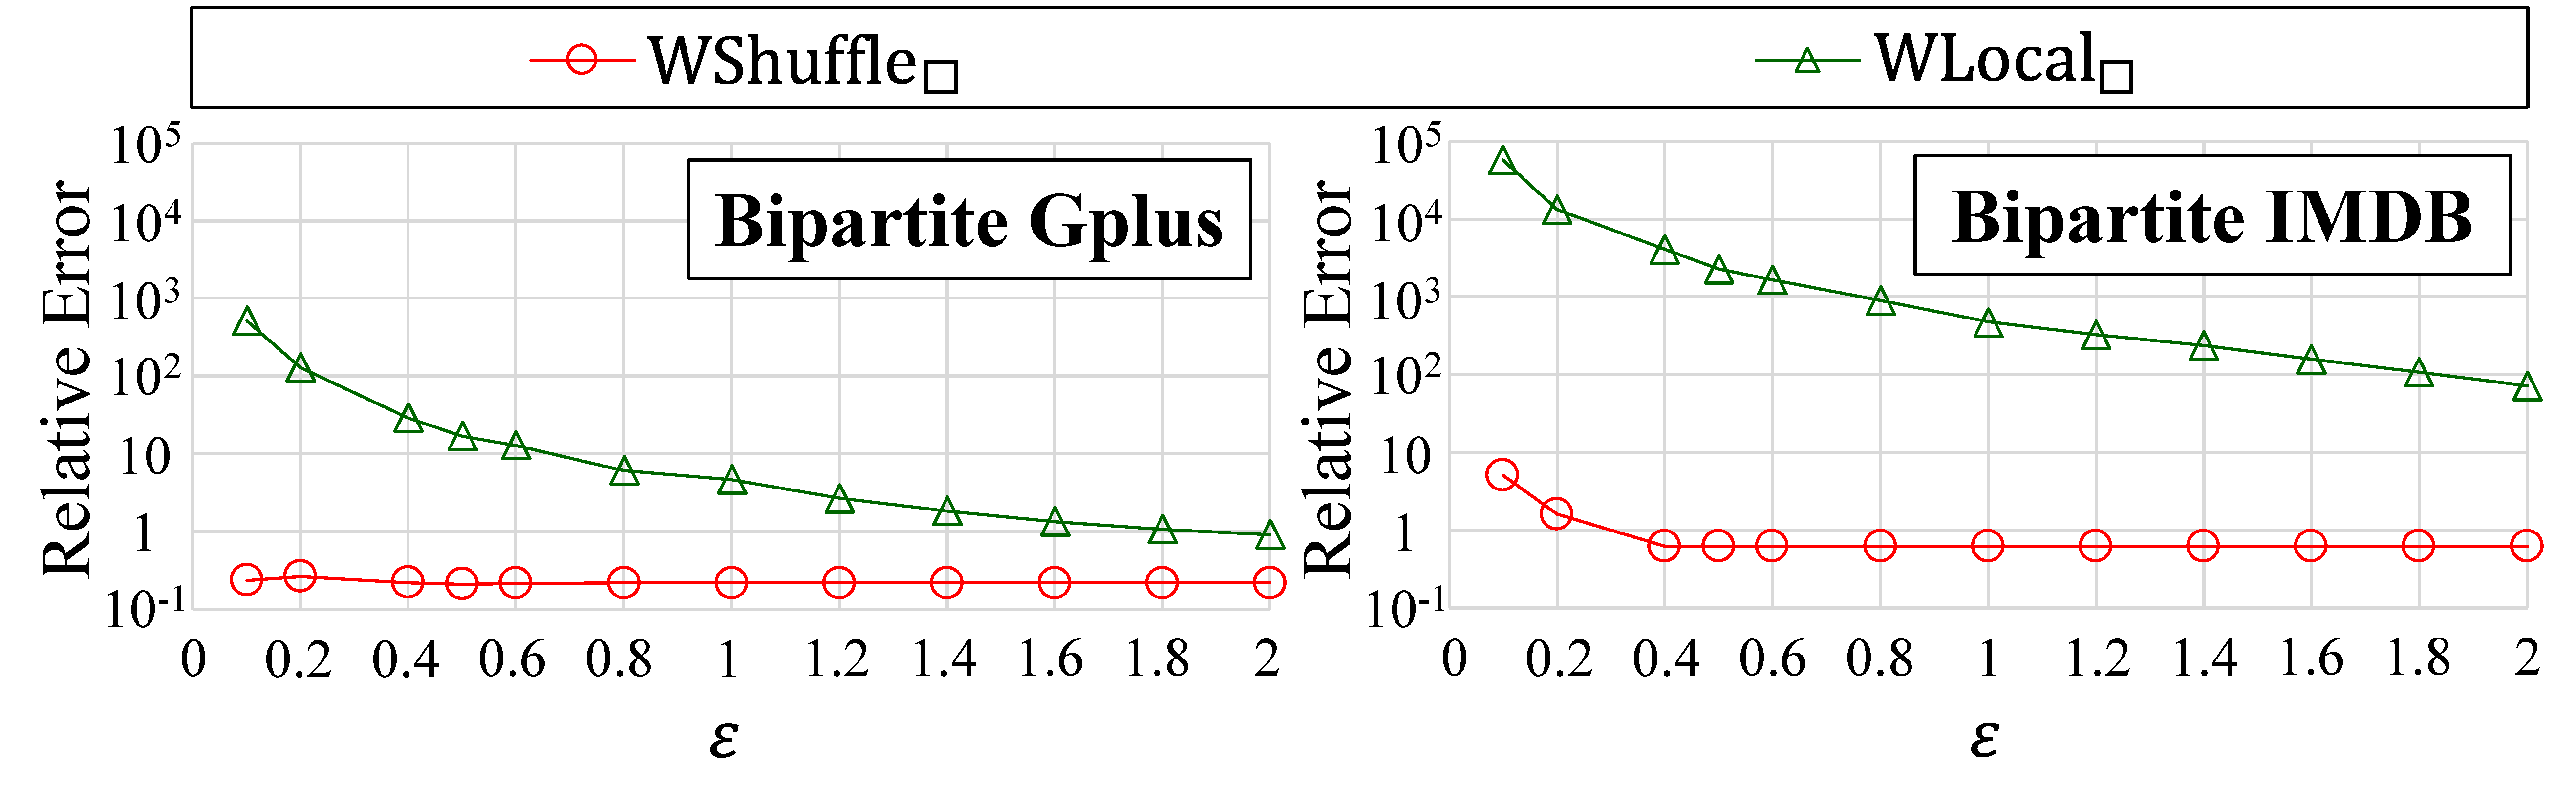
\includegraphics[width=0.99\linewidth]{fig/res8_Bip.pdf}
  
  \caption[Relative error in the bipartite graphs.]{Relative error in the bipartite graph data
  ($n=107614$ in \Gplus{}, $n=896308$ in \IMDB{}, $c=1$).
  }
  \label{chap3-fig:res8_Bip}
%\end{figure}
\vspace{2mm}
%\begin{figure}[t]
  \centering
  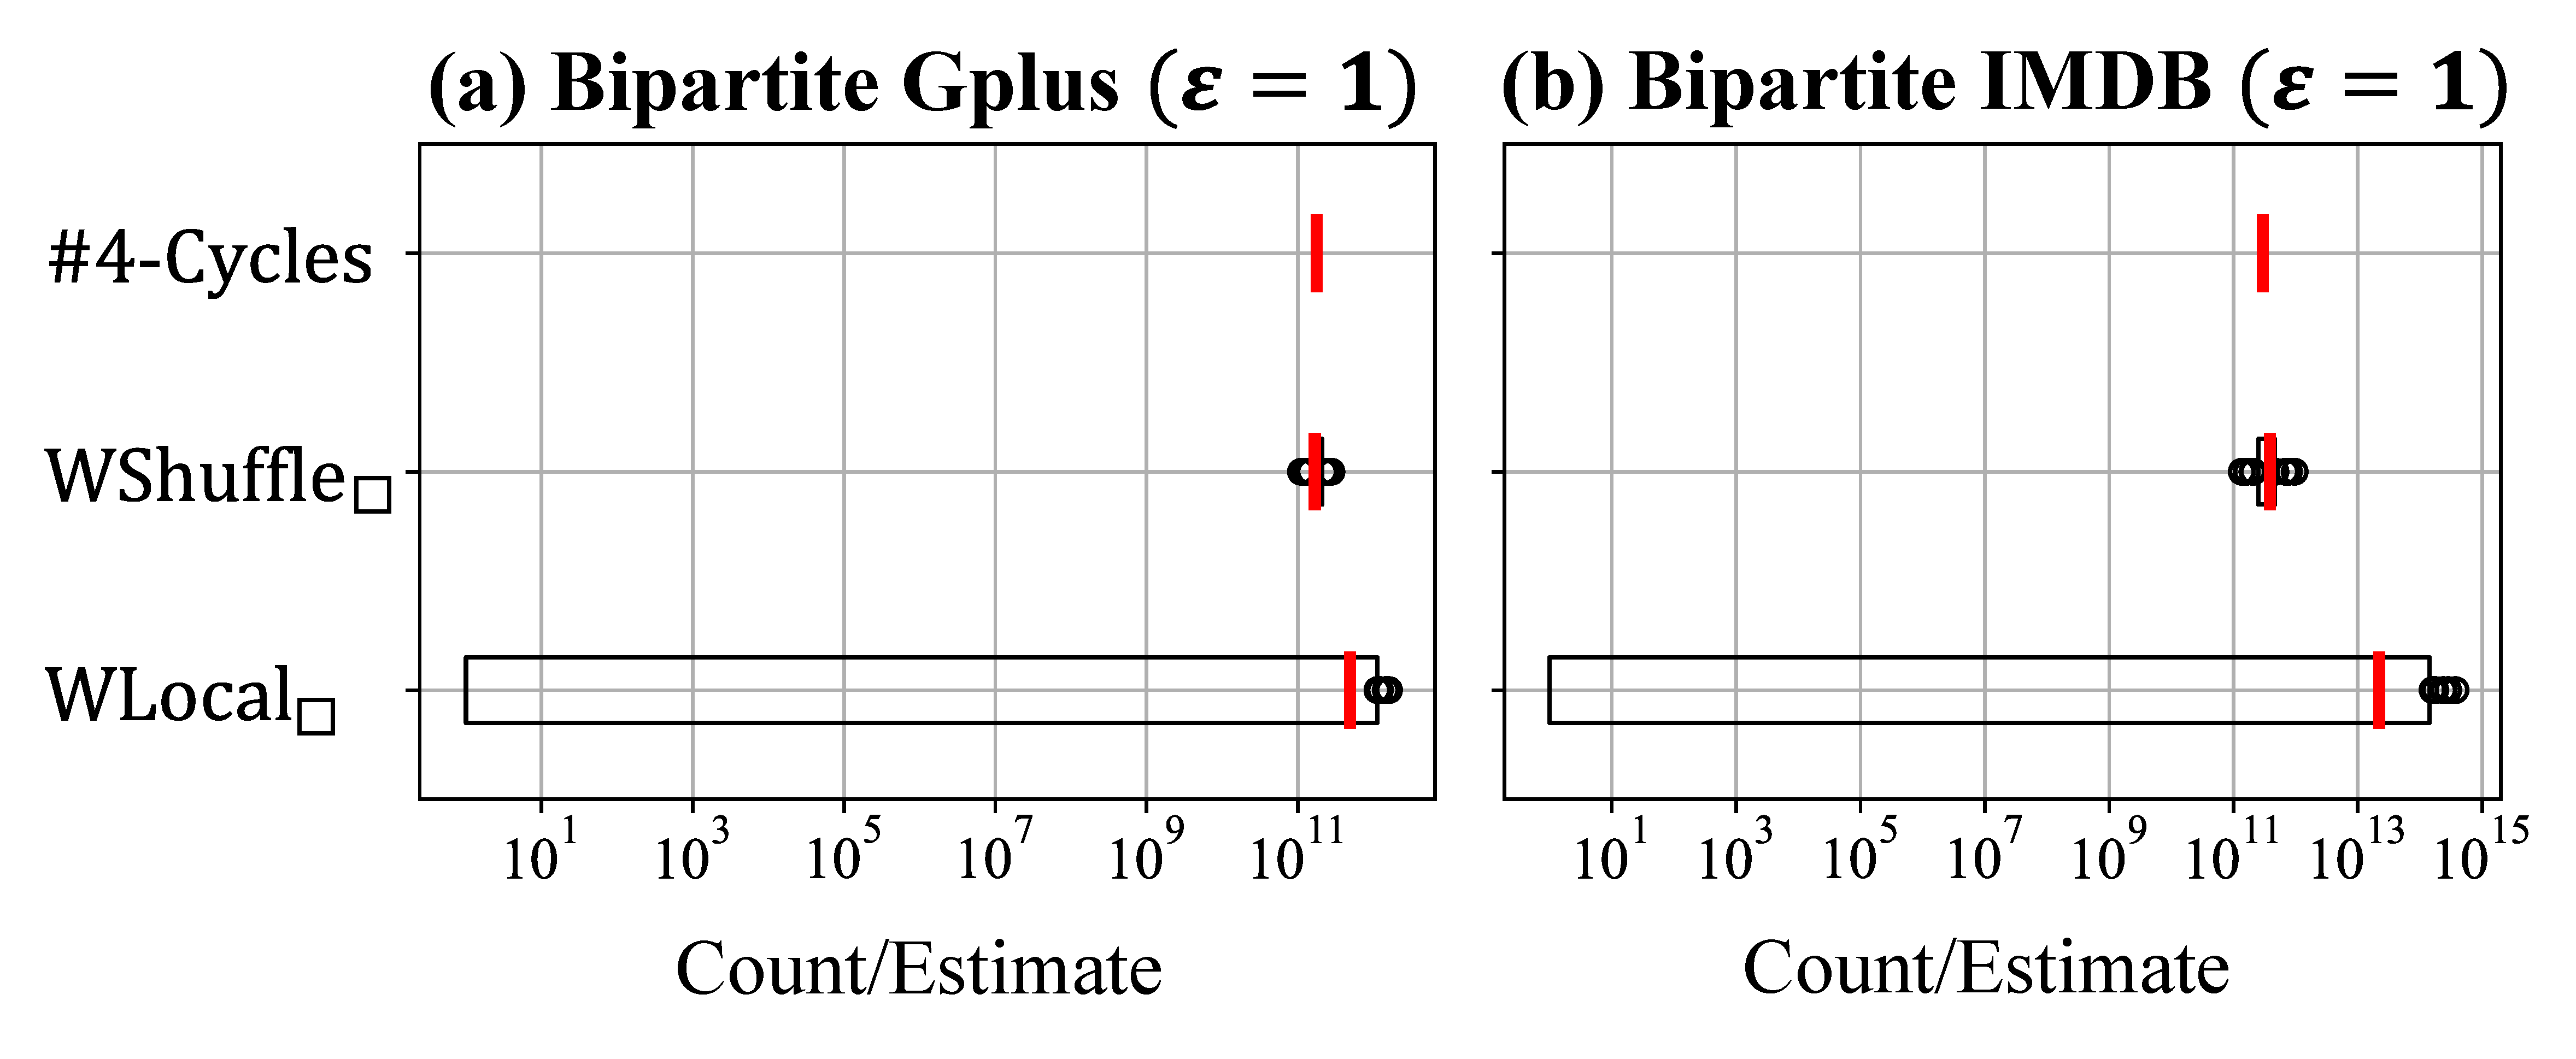
\includegraphics[width=0.92\linewidth]{fig/res8_Bip_box.pdf}
  
  \caption[Box plots of counts/estimates in the bipartite graphs.]{Box plots of counts/estimates in the bipartite graph data
  ($n=107614$ in \Gplus{}, $n=896308$ in \IMDB{}, $c=1$).
  \#4-Cycles represents the true 4-cycle count.
  Each box plot represents the median (red), lower/upper quartile, and outliers (circles) of $20$ estimates.
  The leftmost values are smaller than $1$.
  }
  \label{chap3-fig:res8_Bip_box}
\end{figure}

Figure~\ref{chap3-fig:res8_Bip} shows the results.
We observe that \AlgWSCyc{} significantly outperforms \AlgWLCyc{} in these datasets.
Compared to Figure~\ref{chap3-fig:res1_eps}(b), the relative error of \AlgWSCyc{} is a bit larger in the bipartite graph data.
For example, when $\epsilon=1$, the relative error of \AlgWSCyc{} is $0.147$, $0.308$, $0.217$, and $0.626$ in \Gplus{}, \IMDB{}, the bipartite \Gplus{}, and the bipartite \IMDB{}, respectively.
This is because the 4-cycle count is reduced by removing edges within each group.
In \Gplus{}, the 4-cycle count is reduced from $1.42 \times 10^{12}$ to $1.77 \times 10^{11}$.
In \IMDB{}, it is reduced from $2.37 \times 10^{12}$ to $2.96 \times 10^{11}$.
Consequently, the denominator in the relative error becomes smaller, and the relative error becomes larger.

Although the relative error of \AlgWSCyc{} with $\epsilon=1$ is about $0.6$ in the bipartite \IMDB{}, \AlgWSCyc{} still calculates a rough estimate of the 4-cycle count.
Figure~\ref{chap3-fig:res8_Bip_box} shows box plots of counts or estimates in the bipartite graph data.
This figure shows that \AlgWLCyc{} fails to estimate the 4-cycle count.
In contrast, \AlgWSCyc{} successfully calculates a rough estimate of the 4-cycle count in all cases.

In summary, our \AlgWSCyc{} significantly outperforms \AlgWLCyc{} and accurately counts 4-cycles in the bipartite graphs as well.

\section{Standard Error of the Average Relative Error}
\label{chap3-sec:standard_error}

In Section~\ref{chap3-sec:experiments}, we evaluated the average relative error over $20$ runs for each algorithm. 
In this appendix, we evaluate the standard error of the average relative error. 

\begin{figure}[t]
  \centering
  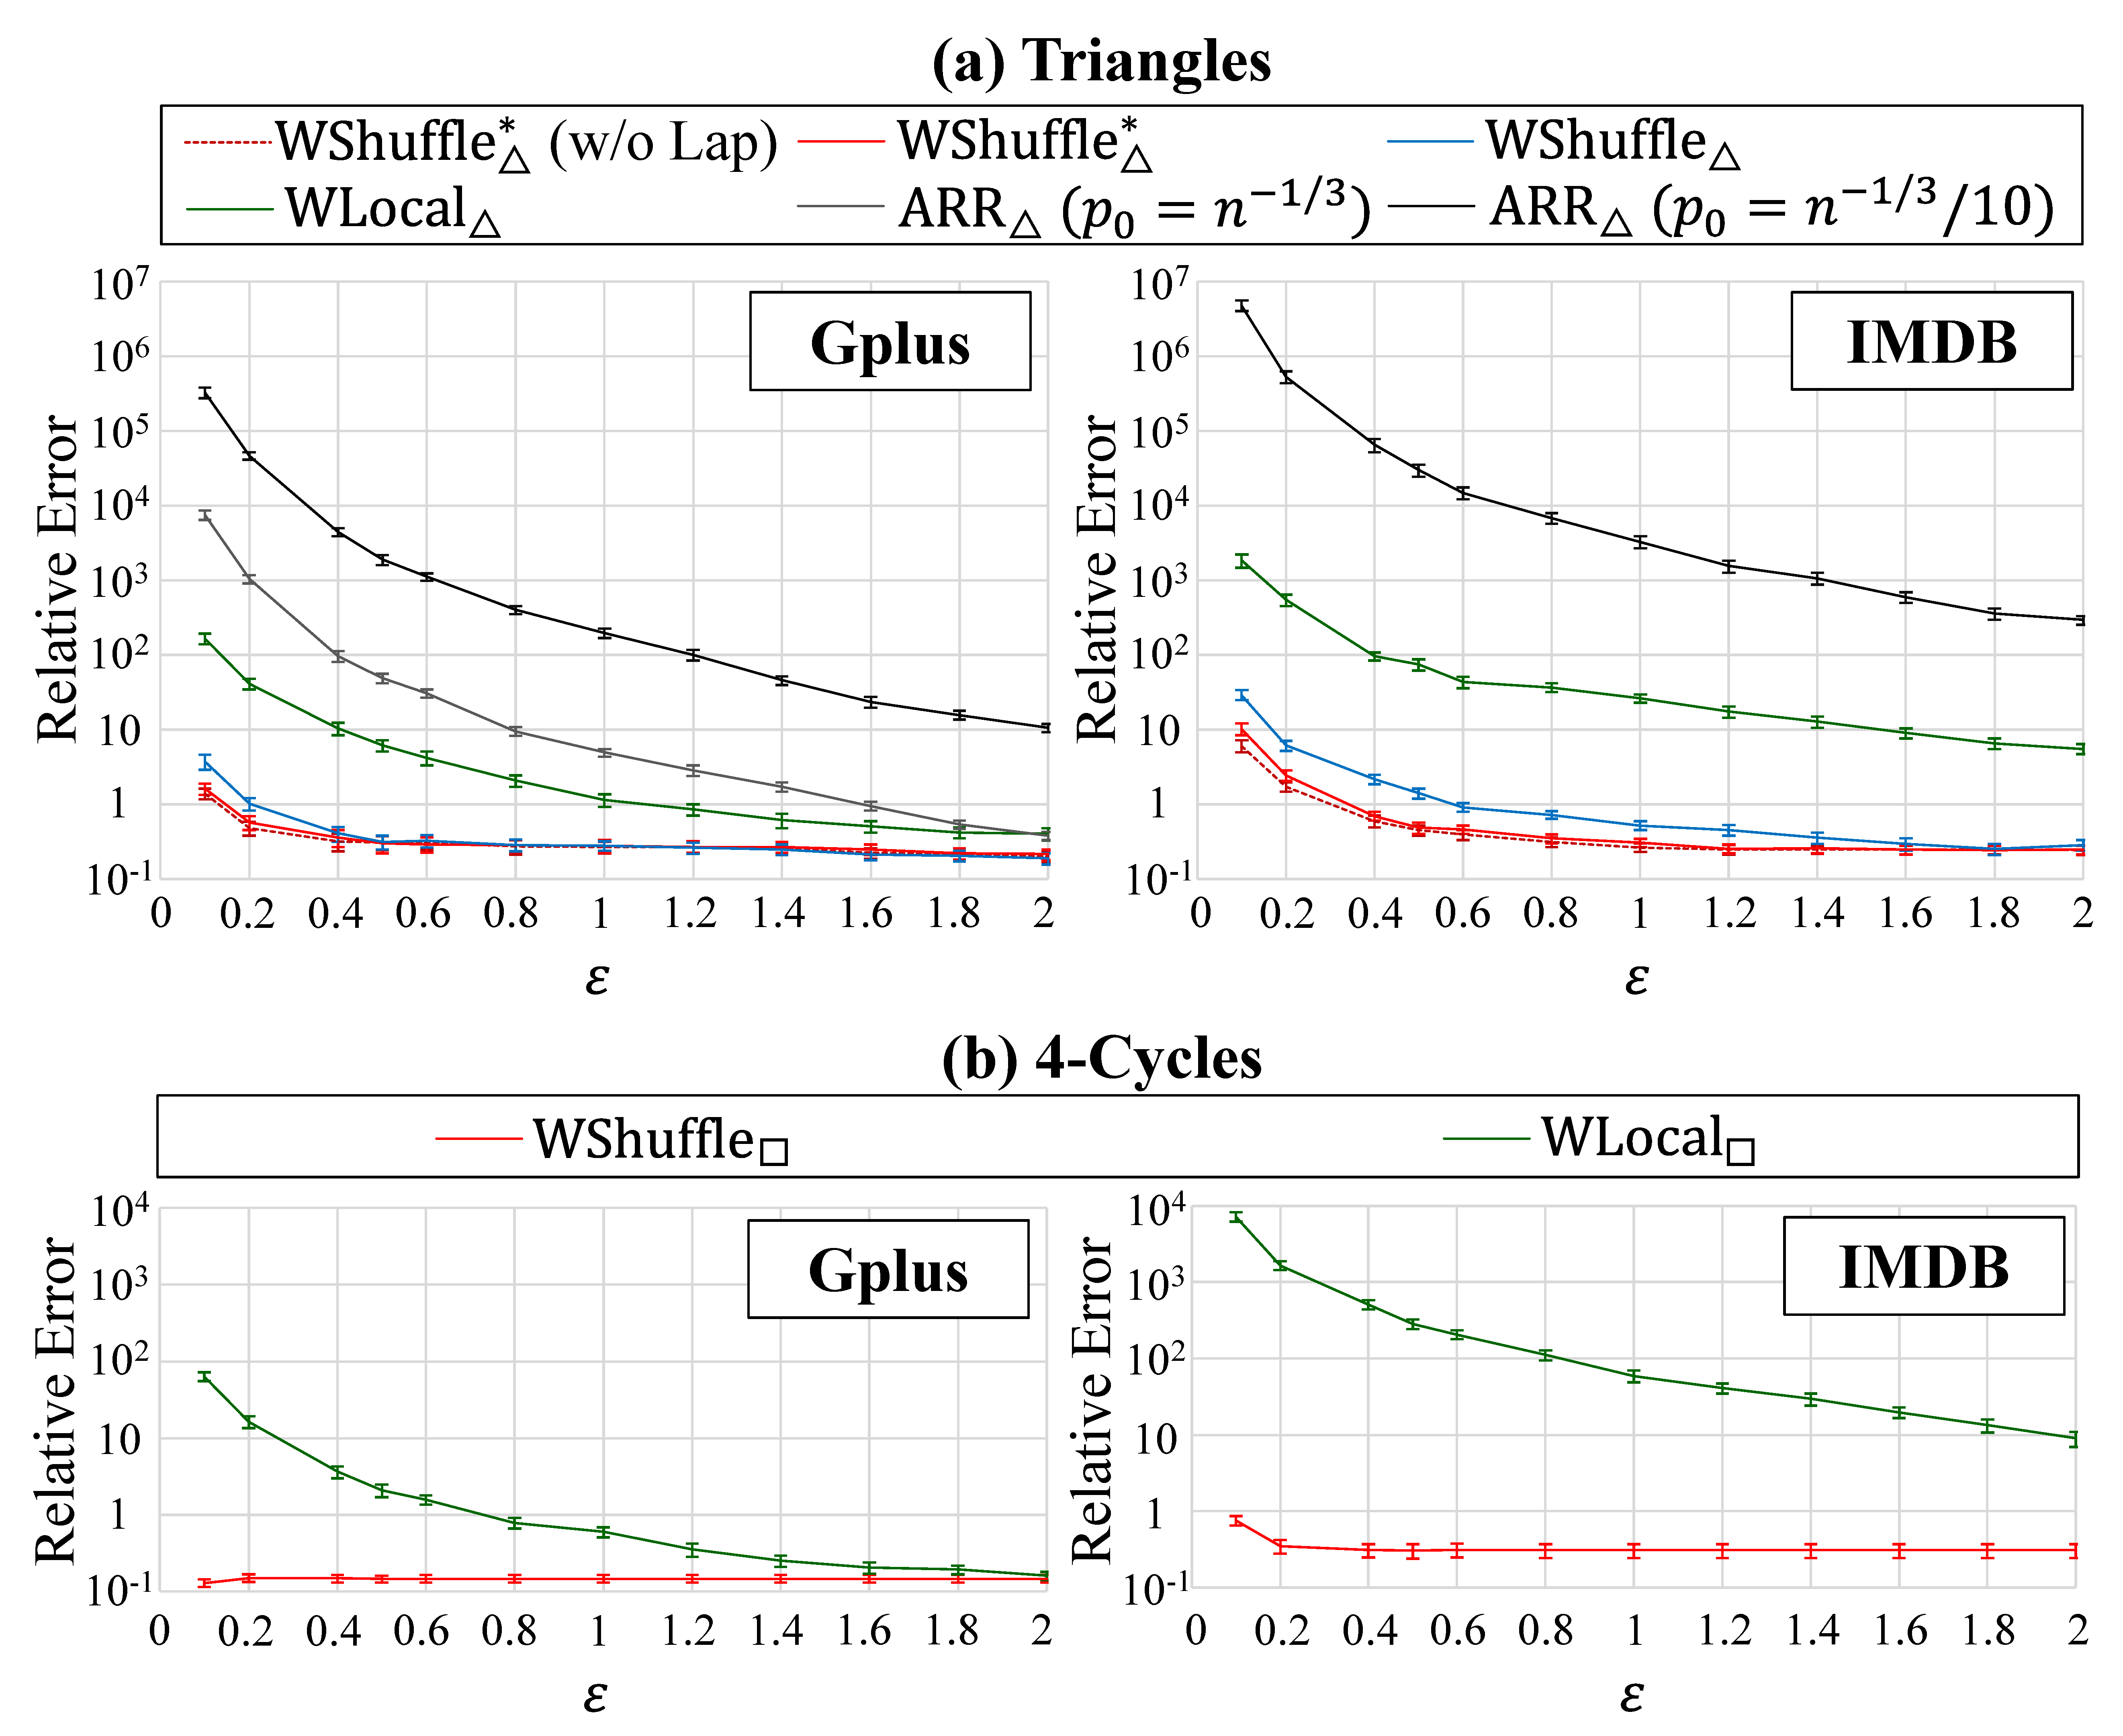
\includegraphics[width=0.99\linewidth]{fig/res9_std_err.pdf}
  
  \caption[Standard of the average relative error.]{Standard error of the average relative error in Figure~\ref{chap3-fig:res1_eps}. 
  Each error bar represents $\pm$ standard error.
  }
  \label{chap3-fig:res9_std_err}
\end{figure}

Figure~\ref{chap3-fig:res9_std_err} shows the standard error of the average relative error in Figure~\ref{chap3-fig:res1_eps}. 
We observe that the standard error is small. 
For example, as shown in Table~\ref{chap3-tab:res1_eps_tri_time} (a), the average relative error of \AlgWSTriVR{} is $0.298$ ($\epsilon=0.5$) or $0.277$ ($\epsilon=1$) in \Gplus{}. 
Figure~\ref{chap3-fig:res9_std_err} shows that the corresponding standard error is $0.078$ ($\epsilon=0.5$) or $0.053$ ($\epsilon=1$). Thus, we conclude that $20$ runs are sufficient in our experiments. 

\section{MSE of the Existing One-Round Local Algorithms}
\label{chap3-sec:upper}
% Upper bounds for the efficient one-round local algorithm in \cite{Imola_USENIX22}. Here, we do not assume the ER model, unlike \cite{Imola_USENIX21}.

Here, we show the MSE of the existing one-round local algorithms \AlgARRTri{} \cite{Imola_USENIX22} and \AlgRRTri{} \cite{Imola_USENIX21}.
Specifically, we prove the MSE of \AlgARRTri{} because \AlgARRTri{} includes \AlgRRTri{} as a special case; i.e., the MSE of \AlgRRTri{} is immediately derived from that of \AlgARRTri{}.

We also note that the MSE of \AlgRRTri{} is proved in \cite{Imola_USENIX21} under the assumption that a graph is generated from the Erd\"os-R\'enyi graph model \cite{NetworkScience}.
However, this assumption does not hold in practice, because the Erd\"os-R\'enyi graph does not have a power-law degree distribution.
In contrast, we prove the MSE of \AlgARRTri{} (hence \AlgRRTri{}) without making any assumption on graphs.

% Below, we briefly explain \AlgARRTri{} and then prove the $l_2$ loss of \AlgARRTri{}.

\smallskip
\noindent{\textbf{Algorithm.}}~~First, we briefly explain \AlgARRTri{}.
In this algorithm, each user $v_i$ obfuscates her neighbor list $\bma_i \in \{0,1\}^n$ using the ARR (Asymmetric Randomized Response) whose input domain and output range are $\{0,1\}$.
%which samples 0/1 after applying the RR.
Specifically, the ARR has two parameters $\epsilon \in \nnreals$ and $\mu \in [0,\frac{e^\epsilon}{e^\epsilon + 1}]$.
% Let $ARR_{\epsilon,\mu}$ be the ARR.
Given $1$ (resp.~$0$), the ARR outputs $1$ with probability $\mu$ (resp.~$\mu e^{-\epsilon}$).
This mechanism is equivalent to $\epsilon$-RR
% Warner's RR
followed by edge sampling, which samples each 1 with probability $p_0$ satisfying $\mu = \frac{e^\epsilon}{e^\epsilon+1} p_0$.
% The ARR provides $\epsilon$-edge LDP.
User $v_i$ applies the ARR to bits $a_{i,1}, \ldots, a_{i,i-1}$ for smaller user IDs in her neighbor list $\bma_i$ (i.e., lower triangular part of $\bmA$) and sends the noisy bits to the data collector.
Then, the data collector constructs a noisy graph $G^*$ based on the noisy bits.

The data collector counts triangles, 2-edges (three nodes with two edges), 1-edge (three nodes with one edge), and no-edges (three nodes with no edges) in the noisy graph $G^*$.
Let $m_3^*, m_2^*, m_1^*, m_0^* \in \nnints$ be the numbers of triangles, 2-edges, 1-edge, and no-edges, respectively, in $G^*$.
Note that $m_3^* + m_2^* + m_1^* + m_0^* = \binom{n}{3}$.
Finally, the data collector estimates the number $f^\triangle(G)$ of triangles as follows:
\begin{align}
    \hf^\triangle(G) = \frac{1}{(e^\epsilon-1)^3}(e^{3\epsilon} \hat{m}_3 - e^{2\epsilon} \hat{m}_2 + e^\epsilon \hat{m}_1 - \hat{m}_0),
    \label{chap3-eq:ARR_hf}
\end{align}
where
\begin{align}
\hat{m}_3 &= \textstyle{\frac{m_3^*}{p_0^3}} \label{chap3-eq:ARR_m3}\\
\hat{m}_2 &= \textstyle{\frac{m_2^*}{p_0^2} - 3(1-p_0)\hat{m}_3} \label{chap3-eq:ARR_m2}\\
\hat{m}_1 &= \textstyle{\frac{m_1^*}{p_0} - 3(1-p_0)^2\hat{m}_3 - 2(1-p_0)\hat{m}_2} \label{chap3-eq:ARR_m1}\\
\hat{m}_0 &= \textstyle{\binom{n}{3} - \hat{m}_3 - \hat{m}_2 - \hat{m}_1}. \label{chap3-eq:ARR_m0}
\end{align}
\AlgRRTri{} is a special case of \AlgARRTri{} where $\mu = \frac{e^\epsilon}{e^\epsilon + 1}$ ($p_0 = 1$), i.e. without edge sampling.

\smallskip
\noindent{\textbf{Privacy and Time Complexity.}}~~The ARR is equivalent to $\epsilon$-RR followed by edge sampling, as explained above.
Therefore, \AlgARRTri{} provides $\epsilon$-edge LDP by the post-processing invariance \cite{DP}.

The time complexity of \AlgARRTri{} is dominated by counting the number $m_3$ of triangles in the noisy graph $G^*$.
The expectation of $m_3$ is upper bounded as $\E[\mu_3^*] \leq \mu^3 n^3$, as each user-pair has an edge in $G^*$ with probability at most $\mu$.
Thus, the time complexity of \AlgARRTri{} can be expressed as $O(\mu^3 n^3)$.
This is $O(n^2)$ when $\mu^3 = O(\frac{1}{n})$.

\smallskip
\noindent{\textbf{MSE.}}~~Below, we analyze the MSE of \AlgARRTri{}.
First, we show that \AlgARRTri{} provides an unbiased estimate\footnote{It is informally explained in \cite{Imola_USENIX22} that the estimate of \AlgARRTri{} is unbiased. We formalize their claim.}:
\begin{theorem}
\label{chap3-thm:unbiased_ARR}
In \AlgARRTri{}, $\E[\hf^\triangle(G)] = f^\triangle(G)$.
\end{theorem}
\begin{proof}
Let $m_3, m_2, m_1, m_0 \in \nnints$ be the numbers of triangles, 2-edges, 1-edge, and no-edges, respectively, in the noisy graph $G'$ obtained by applying only $\epsilon$-RR.
Because the ARR independently samples each edge with probability $p_0$, we have:
\begin{align}
\E[m_3^*] &= p_0^3 m_3 \label{chap3-eq:E_m3*}\\
\E[m_2^*] &= 3 p_0^2 (1 - p_0) m_3 + p_0^2 m_2 \label{chap3-eq:E_m2*}\\
\E[m_1^*] &= 3 p_0 (1 - p_0)^2 m_3 + 2 p_0 (1 - p_0) m_2 + p_0 m_1. \label{chap3-eq:E_m1*}
\end{align}
By (\ref{chap3-eq:ARR_hf}), we have:
\begin{align}
& \E[\hf^\triangle(G)] \nonumber\\
&= \frac{1}{(e^\epsilon-1)^3}(e^{3\epsilon} \E[\hat{m}_3] - e^{2\epsilon} \E[\hat{m}_2] + e^\epsilon \E[\hat{m}_1] - \E[\hat{m}_0]) \nonumber\\
&= \frac{1}{(e^\epsilon-1)^3}(e^{3\epsilon} \E[\hat{m}_3] - e^{2\epsilon} \E[\hat{m}_2] + e^\epsilon \E[\hat{m}_1] - \E[\hat{m}_0]). \label{chap3-eq:E_hf_triangle_G}
\end{align}
By (\ref{chap3-eq:ARR_m3}), (\ref{chap3-eq:ARR_m2}), (\ref{chap3-eq:ARR_m1}), (\ref{chap3-eq:ARR_m0}), (\ref{chap3-eq:E_m3*}), (\ref{chap3-eq:E_m2*}), and (\ref{chap3-eq:E_m1*}), we have:
\begin{align*}
\E[\hat{m}_3]
&= \textstyle{\frac{\E[m_3^*]}{p_0^3}}
= \E[m_3] \\
\E[\hat{m}_2]
&= \textstyle{\frac{\E[m_2^*]}{p_0^2} - 3(1-p_0)\E[\hat{m}_3]} \\
&= 3 (1 - p_0) m_3 + m_2 - 3(1-p_0)m_3 \\
&= \E[m_2] \\
\E[\hat{m}_1]
&= \textstyle{\frac{\E[m_1^*]}{p_0} - 3(1-p_0)^2\E[\hat{m}_3] - 2(1-p_0)\E[\hat{m}_2]} \\
&= 3 (1 - p_0)^2 \E[m_3] + 2 (1 - p_0) \E[m_2] + \E[m_1] \\
& \hspace{3mm} - 3(1-p_0)^2 \E[m_3] - 2(1-p_0) \E[m_2] \\ &= \E[m_1] \\
\E[\hat{m}_0]
&= \textstyle{\binom{n}{3} - \E[\hat{m}_3] - \E[\hat{m}_2] - \E[\hat{m}_1]} \\
&= \textstyle{\binom{n}{3} - \E[m_3] - \E[m_2] - \E[m_1]} \\
&= \E[m_0].
\end{align*}
Thus, the equality (\ref{chap3-eq:E_hf_triangle_G}) can be written as follows:
\begin{align}
& \E[\hf^\triangle(G)] \nonumber\\
&= \frac{1}{(e^\epsilon-1)^3}(e^{3\epsilon} \E[m_3] - e^{2\epsilon} \E[m_2] + e^\epsilon \E[m_1] - \E[m_0]).
\label{chap3-eq:E_hf_traingle_G2}
\end{align}
Finally, we use the following lemma:

\begin{lemma}\label{chap3-lemma:triangle_emp}[Proposition 2 in \cite{Imola_USENIX21}]
  \begin{align}
      \textstyle{\mathbb{E}\left[ \frac{e^{3\epsilon}}{(e^\epsilon-1)^3} m_3 \hspace{-0.5mm}-\hspace{-0.5mm} \frac{e^{2\epsilon}}{(e^\epsilon-1)^3} m_2 \hspace{-0.5mm}+\hspace{-0.5mm} \frac{e^\epsilon}{(e^\epsilon-1)^3} m_1 \hspace{-0.5mm}-\hspace{-0.5mm} \frac{1}{(e^\epsilon-1)^3} m_0 \right] \hspace{-0.5mm} = \hspace{-0.5mm} f_\triangle(G).}
      \label{chap3-eq:triangle_emp}
  \end{align}
\end{lemma}
See \cite{Imola_USENIX21} for the proof of Lemma~\ref{chap3-lemma:triangle_emp}.
By (\ref{chap3-eq:E_hf_traingle_G2}) and Lemma~\ref{chap3-lemma:triangle_emp}, we have $\E[\hf^\triangle(G)] = f_\triangle(G)$.
\end{proof}

Next, we show the MSE ($=$ variance) of \AlgARRTri{}:
\begin{theorem}
\label{chap3-thm:var_ARR}
% Let $d_3 = \frac{e^{3\epsilon}}{(e^\epsilon-1)^3}$, $d_2 = \frac{e^{2\epsilon}}{(e^\epsilon-1)^3}$,
% $d_1 = \frac{e^{\epsilon}}{(e^\epsilon-1)^3}$, and
% $d_0 = \frac{1}{(e^\epsilon-1)^3}$.
% Then,
When we treat $\epsilon$ as a constant,
\AlgARRTri{} provides the following utility guarantee:
\begin{align*}
& \MSE(\hf^\triangle(G)) = \V[\hf^\triangle(G)] = O\left(\frac{n^4}{\mu^6}\right).
% & \leq (d_3^2 + d_2^2 + d_1^2 + d_0^2 + 8(d_3 d_2 + d_3 d_1 + d_3 d_0+ d_2 d_1 + d_2 d_0 + d_1 d_0)
% \label{chap3-eq:thm:l2_ARR}
\end{align*}
\end{theorem}
By Theorem~\ref{chap3-thm:var_ARR}, the MSE of \AlgARRTri{} is $O(n^6)$ when we set $\mu^3=O(\frac{1}{n})$ so that the time complexity is $O(n^2)$.
The MSE of \AlgRRTri{} ($\mu=1$) is $O(n^4)$.
Below, we prove Theorem~\ref{chap3-thm:var_ARR}.

\begin{proof}
Let $d_3 = \frac{e^{3\epsilon}}{(e^\epsilon-1)^3}$, $d_2 = - \frac{e^{2\epsilon}}{(e^\epsilon-1)^3}$,
$d_1 = \frac{e^{\epsilon}}{(e^\epsilon-1)^3}$, and
$d_0 = - \frac{1}{(e^\epsilon-1)^3}$.
Then, by (\ref{chap3-eq:ARR_hf}), we have:
% the variance of $\hf^\triangle(G)$ can be expressed as follows:
\begin{align}
    \V[\hf^\triangle(G)]
    &= \V[d_3 \hat{m}_3 + d_2 \hat{m}_2 + d_1 \hat{m}_1 + d_0 \hat{m}_0] \nonumber\\
    &= d_3^2 \V[\hat{m}_3] + d_2^2 \V[\hat{m}_2] + d_1^2 \V[\hat{m}_1] + d_0^2 \V[\hat{m}_0] \nonumber\\
    & \hspace{3mm} + \sum_{i \ne j} d_i d_j \cov(\hat{m}_i, \hat{m}_j).
    \label{chap3-eq:V_hf_cov}
\end{align}
By the Cauchy-Schwarz inequality,
\begin{align}
|\cov(\hat{m}_i, \hat{m}_j)|
&\leq \sqrt{\V[\hat{m}_i]\V[\hat{m}_j]} \nonumber\\
&\leq \max\{\V[\hat{m}_i], \V[\hat{m}_j]\} \nonumber\\
&\leq \V[\hat{m}_i] + \V[\hat{m}_j].
\label{chap3-eq:cov_hm_ij}
\end{align}
Therefore, we have:
\begin{align}
    \V[\hf^\triangle(G)]
    %&\leq (d_3^2 + 2d_3(d_2 + d_1 + d_0)) \V[\hat{m}_3] \nonumber\\
    %&\hspace{4mm} + (d_2^2 + 2d_2(d_3 + d_1 + d_0)) \V[\hat{m}_2] \nonumber\\
    %&\hspace{4mm} + (d_1^2 + 2d_1(d_3 + d_2 + d_0)) \V[\hat{m}_1] \nonumber\\
    %&\hspace{4mm} + (d_0^2 + 2d_0(d_3 + d_2 + d_1)) \V[\hat{m}_0] \nonumber\\
    = O(\V[\hat{m}_3] + \V[\hat{m}_2] + \V[\hat{m}_1] + \V[\hat{m}_0]).
    \label{chap3-eq:V_hf_m3210}
\end{align}

Below, we upper bound $\V[\hf^\triangle(G)]$ in (\ref{chap3-eq:V_hf_m3210}) by bounding $\V[m_3^*], \ldots, \allowbreak \V[m_0^*]$ and then $\V[\hat{m}_3], \ldots, \allowbreak \V[\hat{m}_0]$.
Let $T_{i,j,k} \in \{0,1\}$ be a random variable that takes $1$ if and only if $v_i$, $v_j$, and $v_k$ form a triangle in the noisy graph $G^*$.
Then we have:
\begin{align*}
    \V[m_3^*]
    &= \V\left[\sum_{i,j,k} T_{i,j,k}\right] \\
    &= \sum_{i<j<k} \sum_{i'<j'<k'} \cov[T_{i,j,k}, T_{i',j',k'}].
%    &\leq \binom{n}{3} + \binom{n}{2} (n-2)(n-3).
\end{align*}
%The last inequality holds because
If $v_i, v_j, v_k$ and $v_{i'}, v_{j'}, v_{k'}$ intersect in zero or one node, then $T_{i,j,k}$ and $T_{i',j',k'}$ are independent
%Thus, the covariance $\cov[T_{i,j,k}, T_{i',j',k'}]$ is not 0 only if the two triplets intersect in two or three nodes.
and their covariance is $0$.
There are only $O(n^4)$ choices of $v_i, v_j, v_k$ and $v_{i'}, v_{j'}, v_{k'}$ that intersect in two or more nodes, as there can only be $4$ distinct nodes.
Therefore, we have $\V[m_3^*] = O(n^4)$.
Similarly, we can prove $\V[m_2^*] = \V[m_1^*] = \V[m_0^*] = O(n^4)$ by regarding $T_{i,j,k}$ as a random variable that takes $1$ if and only if $v_i$, $v_j$, and $v_k$ form a 2-edge, 1-edge, and no-edges, respectively.
In summary, we have:
\begin{align}
    \V[m_3^*] = \V[m_2^*] = \V[m_1^*] = \V[m_0^*] = O(n^4).
    \label{chap3-eq:V_m3210_ast}
\end{align}
By (\ref{chap3-eq:V_m3210_ast}) and $\mu = \frac{e^\epsilon}{e^\epsilon+1} p_0$, we can upper bound the variance of $\hat{m}_3$ in (\ref{chap3-eq:ARR_m3}) as follows:
\begin{align*}
    \V[\hat{m}_3]
    = \frac{\V[m_3^*]}{p_0^6}
    = O\left(\frac{n^4}{\mu^6}\right).
\end{align*}
As with (\ref{chap3-eq:V_hf_cov}), (\ref{chap3-eq:cov_hm_ij}), and (\ref{chap3-eq:V_hf_m3210}), we can upper bound the variance of $\hat{m}_2$ in (\ref{chap3-eq:ARR_m2}) by using the Cauchy-Schwarz inequality as follows:
\begin{align*}
    & \V[\hat{m}_2] \\
    &= \textstyle{\V\left[\frac{m_2^*}{p_0^2} - \frac{3(1-p_0)}{p_0^3}m_3^*\right]} \\
    &= \frac{\V[m_2^*]}{p_0^4} + \frac{9(1-p_0)^2\V[m_3^*]}{p_0^6} - \frac{6(1-p_0)\cov(m_2^*,m_3^*)}{p_0^5} \\
    &\leq \frac{\V[m_2^*]}{p_0^4} + \frac{9(1-p_0)^2\V[m_3^*]}{p_0^6} + \frac{6(1-p_0)(\V[m_2^*]+\V[m_3^*])}{p_0^5} \\
    &= O\left(\frac{n^4}{\mu^6}\right) \\
    % \V[\hat{m}_1]
    % &= \V\left[\frac{m_1^*}{p_0} + \frac{3(1-p_0)^2}{p_0^3}m_3^* - \frac{2(1-p_0)}{p_0^2}m_2^* \right] \\
    % &= O\left(\frac{n^4}{\mu^6}\right) \\
    % \V[\hat{m}_0]
    % &= \V\left[\frac{m_3^*}{p_0^3} + \frac{3(1-p_0)^2}{p_0^3}m_3^* - \frac{2(1-p_0)}{p_0^2}m_2^* \right] \\
    % &= O\left(\frac{n^4}{\mu^6}\right) \\
\end{align*}
Similarly, we have
%$\V[\hat{m}_1] = \V[\hat{m}_0] =  O\left(\frac{n^4}{\mu^6}\right)$.
\begin{align*}
    &\V[\hat{m}_1] \\
    &= \textstyle{\V\left[\frac{m_1^*}{p_0} + \frac{3(1-p_0)^2}{p_0^3}m_3^* - \frac{2(1-p_0)}{p_0^2}m_2^* \right]} \\
    &= O\left(\frac{n^4}{\mu^6}\right) \\
    &\V[\hat{m}_0] \\
    &= \V[\hat{m}_3 + \hat{m}_2 + \hat{m}_1]\\
    &=
    \textstyle{\V\left[\frac{m_3^*}{p_0^3}
    + \frac{m_2^*}{p_0^2} - \frac{3(1-p_0)}{p_0^3}m_3^*
    + \frac{m_1^*}{p_0} + \frac{3(1-p_0)^2}{p_0^3}m_3^* - \frac{2(1-p_0)}{p_0^2}m_2^*
     \right]} \\
    &= O\left(\frac{n^4}{\mu^6}\right).
\end{align*}
In summary,
\begin{align}
    \V[\hat{m}_3] = \V[\hat{m}_2] = \V[\hat{m}_1] = \V[\hat{m}_0] = O\left(\frac{n^4}{\mu^6}\right).
    \label{chap3-eq:V_hm3210}
\end{align}
By (\ref{chap3-eq:V_hf_m3210}) and (\ref{chap3-eq:V_hm3210}),
$\V[\hf^\triangle(G)] = O\left(\frac{n^4}{\mu^6}\right)$.
\end{proof}

% \section{Proofs of Statements in Section~\ref{chap3-sec:triangle}}
\section{Proofs of Statements in Section 5}
\label{chap3-sec:triangle_proof}
% Below, we provide proofs of statements in Section~\ref{chap3-sec:triangle}.
% Hereinafter, a subscript $r$ in $\E_r$, $\V_r$, or $\cov_r$ represents that $\E$, $\V^+$, or $\cov$ is taken over $r$.

% \subsection{Proof of Theorem~\ref{chap3-thm:DP_I}}
% \label{chap3-sub:DP_I_proof}
% TBD
For these proofs, we will write $f_{i,\sigma}(G)$ as a shorthand for
$f_{\sigma(i), \sigma(i+1)}$ and $\hf_{i,\sigma}(G)$ as a shorthand for
$\hf_{\sigma(i), \sigma(i+1)}$.

\subsection{Proof of Theorem~\ref{chap3-thm:unbiased_I}}
\label{chap3-sub:unbiased_I_proof}
    From~\eqref{chap3-eq:hfij_triangle}, the quantity $\hf_{i,j}^\triangle(G)$ can be written as follows:
    \begin{align}
        \hf_{i,j}^\triangle(G)
        &= \frac{1}{2} (\hf_{i,j}^{(1)}(G) + \hf_{i,j}^{(2)}(G)),
        \label{chap3-eq:est_decomp}
    \end{align}
    where
    \begin{align}
        \hf_{i,j}^{(1)}(G)
        &= \frac{(z_{i,j}-q)\sum_{k \in I_{-(i,j)}} (y_{k} - q_L)}{(1-2q)(1-2q_L)} \label{chap3-eq:est1}\\
        \hf_{i,j}^{(2)}(G))
        &= \frac{(z_{j,i}-q)\sum_{k \in I_{-(i,j)}} (y_{k} - q_L)}{(1-2q)(1-2q_L)}, \label{chap3-eq:est2}
    \end{align}
    and each variable $y_k$ represents the output of the RR for the existence of wedge $w_{i-k-j}$ (see Algorithm~\ref{chap3-alg:WShuffle}).
    We call $\hf_{i,j}^{(1)}(G)$ and $\hf_{i,j}^{(2)}(G)$ the first and second estimates, respectively.

    \smallskip
    \noindent{\textbf{First Estimate.}}~~Since variables $z_{i,j}$ and $y_{k}$ in~\eqref{chap3-eq:est1} are independent, we have
    \begin{equation*}
        \E[\hf_{i,j}^{(1)}(G)] = \frac{\E[z_{i,j}-q]\sum_{k \in I_{-(i,j)}}
        \E[y_{k} - q_L]}{(1-2q)(1-2q_L)}.
    \end{equation*}
    First, suppose $(v_i,v_j) \notin E$. Then, $z_{i,j} = 1$ with probability $q$, and $\E[z_{i,j} - q] = 0$. This means $\E[\hf_{i,j}^{(1)}(G)] = f_{i,j}^\triangle(G) = 0$.
    Second, suppose $(v_i,v_j) \in E$. We have $z_{i,j}=1$ with probability $1-q$.
    We have $\E[z_{i,j} - q] = 1-2q$. For any $k \in I_{-(i,j)}$, if
    $w_{i-k-j} = 0$, then we have $\E[y_{k} - q_L] = 0$. If
    $w_{i-k-j} = 1$, then $\E[y_{k}-q_L] = 1-2q_L$. Written concisely, we
    can say $\E[y_{k}-q_L] = (1-2q_L)w_{i-k-j}$. Putting this together, we have
    \begin{align*}
        \E[\hf_{i,j}^{(1)}(G)] &= \frac{(1-2q)\sum_{k \in
        I_{-(i,j)}}(1-2q_L)w_{i-k-j}}{(1-2q)(1-2q_L)} \\
        &= \sum_{k \in I_{-(i,j)}} w_{i-k-j} \\
        &= f_{i,j}^\triangle(G).
    \end{align*}
    Thus, $\E[\hf_{i,j}^{(1)}(G)] = f_{i,j}^\triangle(G)$ holds for both cases.

    \smallskip
    \noindent{\textbf{Second and Average Estimates.}}~~Similarly, we can prove that $\E[\hf_{i,j}^{(2)}(G)] = f_{i,j}^\triangle(G)$ holds.
    Then, by (\ref{chap3-eq:est_decomp}), $\E[\hf_{i,j}^\triangle(G)] = f_{i,j}^\triangle(G)$ holds. \qed

\subsection{Proof of Theorem~\ref{chap3-thm:l2-loss_I}}
\label{chap3-sub:l2-loss_I_proof}

Recall that $\hf_{i,j}^\triangle(G)$ is an average of the first estimate $\hf_{i,j}^{(1)}(G)$ and second estimate $\hf_{i,j}^{(2)}(G)$; see (\ref{chap3-eq:est_decomp}), (\ref{chap3-eq:est1}), and (\ref{chap3-eq:est2}). We bound the variance of the first estimate.

\smallskip
\noindent{\textbf{First Estimate.}}~~Let $H = (z_{i,j}-q)\sum_{k \in I_{-(i,j)}} (y_{k} - q_L)$.
Using the law of total variance, we have
\begin{align*}
    &\V[\hf_{i,j}^{(1)}(G)] \\
    &= \frac{1}{(1-2q)^2(1-2q_L)^2}\left(\E_z[\V_y[H | z_{i,j}]] + \V_z[\E_y[H | z_{i,j}]]\right),
\end{align*}
where $\E_z$ (resp.~$\E_y$) represents the expectation over $z_{i,j}$ (resp.~$y_{k}$).
$\V_z$ (resp.~$\V_y$) represents the variance over $z_{i,j}$ (resp.~$y_{k}$).

We upper bound $\V_z[\E_y[H | z_{i,j}]]$ first. Let $E_y = \E_y[\sum_{k \in
I_{-(i,j)}} y_{k} \allowbreak -q_L]$. When $z_{i,j} = 0$, we have
\begin{align*}
\E_y[H] &= -q\E_y[\textstyle{\sum_{k \in I_{-(i,j)}} y_{k}-q_L}] = -qE_y.
\end{align*}
When $z_{i,j} = 1$, we have
\[
  \E_y[H] = (1-q)\E_y[\textstyle{\sum_{k \in I_{-(i,j)}} y_{k}-q_L}] = (1-q)E_y.
\]
The difference between these two quantities is $E_y$.
Since $z_{i,j}$ is a Bernoulli random variable with bias $q$ on either $0$ or
$1$, we have $\V_z[\E_y[H|z_{i,j}]] = E_y^2 q(1-q)$.
% \leq E_y^2(1-q)$.
Recalling that $\E_y[y_{k}-q_L] = (1-2q_L)w_{i-k-j}$ (see the proof of Theorem~\ref{chap3-thm:unbiased_I}), by linearity of expectation we have that
\begin{align*}
    E_y &= \sum_{k \in I_{-(i,j)}} (1-2q_L)w_{i-k-j} \\
    &\leq (1-2q_L) d_{max}.
\end{align*}
Thus,
\[
  \V_z[\E_y[H|z_{i,j}]] \leq q(1-2q_L)^2 d_{max}^2.
\]

Now, we upper bound $\E_z[\V_y[H | z_{i,j}]]$. When $z_{i,j} = 0$, we have $H =
-q \sum_{k \in I_{-(i,j)}} (y_{k}-q)$, which is a sum of $n-2$ Bernoulli random variables.
% , each with bias $q_L$.
Thus, $\V_y[H | z_{i,j}] = q^2 (n-2) q_L(1-q_L) \leq q^2 q_L n$. When $z_{i,j} = 1$, we have
by a similar argument that $\V_y[H | z_{i,j}] \leq (1-q)^2 q_L n$. Regardless of the value
of $z_{i,j}$, both values attainable by $\V_y[H | z_{i,j}]$ are at most $nq_L$.
Thus,
\[
\E_z[\V_y[H | z_{i,j}]] \leq n q_L.
\]

Putting all this together, we have the following upper-bound:
\[
  \V[\hf_{i,j}^{(1)}(G)] \leq \frac{n q_L + q(1-2q_L)^2 d_{max}^2}{(1-2q)^2(1-2q_L)^2}.
\]

\smallskip
\noindent{\textbf{Second and Average Estimates.}}~~Similarly, we can prove the same upper-bound for the second estimate $\hf_{i,j}^{(2)}(G)$.
Using~\eqref{chap3-eq:est_decomp} and Lemma~\ref{chap3-lem:var-sum} at the end of Appendix~\ref{chap3-sub:l2-loss_I_proof}, we have
$\V[\hf_{i,j}^\triangle(G)] \leq \V[\hf_{i,j}^{(1)}(G)]$, and the result follows.

\smallskip
\noindent{\textbf{Effect of Shuffling.}}~~When $\epsilon$ and $\delta$ are constants
and $\epsilon_L \geq \log n + O(1)$, we
have $nq_L = \frac{n}{e^{\epsilon_L} + 1} = O(1)$ and
$q_L = O(1/n)$,
%$(1-2q_L)^2 \geq 0.5$,
and the bound becomes
\[
  \V[\hf_{i,j}^\triangle(G)] \leq O(d_{max}^2).
\]\qed

\begin{lemma}\label{chap3-lem:var-sum}
  Let $X,Y$ be two real-valued random variables. Then $\V[X+Y] \leq 4\max\{\V[X], \V[Y]\}$.
\end{lemma}
\begin{proof}
  We have $\V[X+Y] = \V[X] + \V[Y] + 2Cov(X,Y)$. By the Cauchy-Schwarz
  inequality, we have $Cov(X,Y) \leq \sqrt{\V[X]\V[Y]} \leq \max\{\V[X],
  \V[Y]\}$. Our result follows by observing $\V[X] + \V[Y] \leq 2\max\{\V[X],
  \V[Y]\}$.
\end{proof}
\subsection{Proof of Theorem~\ref{chap3-thm:DP_II}}
\label{chap3-sub:DP_II_proof}
First, we show that $\AlgWSLE{}$ meets the desired privacy requirements.
Let $x_k = w_{i-k-j}$. In step 1 of \AlgWSLE{},
for each $k \in I_{-(i,j)}$, user $v_k$
sends $y_k = \calR_{\epsilon_L}^W(x_k)$ to the shuffler.
Then, the shuffler sends $\{y_{\pi(k)} | k \in I_{-(i,j)}\}$ to the data collector.
Thus, by Theorem~\ref{chap3-thm:shuffle},
$\{x_k | k \in I_{-(i,j)}\}$
is protected with $(\epsilon, \delta)$-DP, where $\epsilon = f(n-2, \epsilon_L, \delta)$.
Note that changing $a_{k,i}$ will change $x_k$ if and only if $a_{k,j} = 1$.
Thus, for any $k \in I_{-(i,j)}$, $a_{k,i}$ and $a_{k,j}$ are protected with $(\epsilon, \delta)$-DP.

In step 1, user $v_i$ (resp.~$v_j$) sends $z_{i,j} = \calR_{\epsilon}^W(a_{i,j})$ (resp.~$z_{j,i} = \calR_{\epsilon}^W(a_{j,i})$) to the data collector.
Since $\calR_{\epsilon}^W$ provides $\epsilon$-DP, $a_{i,j}$ and $a_{j,i}$ are protected with $\epsilon$-DP.

Putting all this together, each element of the $i$-th and $j$-th columns in the adjacency matrix $\bmA$ is protected with $(\epsilon, \delta)$-DP.
% Thus, Algorithm I provides $(\epsilon, \delta)$-element-level DP.
% Since adding or removing one edge affects at most one element in the $i$-th and $j$-th columns of $\bmA$,
Thus, by Proposition~\ref{chap3-prop:element_edge_DP},
%Algorithm I
\AlgWSLE{}
provides $(\epsilon, \delta)$-element-level DP and ($2\epsilon, 2\delta$)-edge DP.

\AlgWSTri{} interacts with $\bmA$ by calling \AlgWSLE{} on \[(v_{\sigma(1)},
v_{\sigma(2)}), \ldots, (v_{\sigma(2t-1)}, v_{\sigma(2t)}).\] Each of these calls
use disjoint elements of $\bmA$, and thus each element of $\bmA$ is still
protected by $(\epsilon, \delta)$-level DP and by $(2\epsilon, 2\delta)$-edge
DP.\qed

\subsection{Proof of Theorem~\ref{chap3-thm:unbiased_II}}
\label{chap3-sub:unbiased_II_proof}
Notice that the number of triangles in a graph can be computed as
\begin{align}
  6f^\triangle(G) &= \sum_{1 \leq i,j \leq n, i\neq j} f^\triangle_{i,j}(G)
  \nonumber \\
  &= n(n-1) \E_{\sigma}[f^\triangle_{i,
  \sigma}(G)],\label{chap3-eq:triangle-sample-est}
\end{align}
where $i \in [n]$ is arbitrary and $\sigma$ is a random permutation on
$[n]$. The constant $6$ appears because each triangle
appears six times when summing up $f^\triangle_{i,j}(G)$; e.g., a triangle $(v_1, v_2, v_3)$ appears in $f^\triangle_{1,2}(G)$, $f^\triangle_{2,1}(G)$,
$f^\triangle_{1,3}(G)$,
$f^\triangle_{3,1}(G)$,
$f^\triangle_{2,3}(G)$, and
$f^\triangle_{3,2}(G)$.
%is part of $6$ ordered pairs of nodes $(v_i,v_j)$.

Note that there are two kinds of randomness in $\hf^\triangle(G)$: randomness in
choosing a permutation $\sigma$ and randomness in Warner's RR.
By~\eqref{chap3-eq:hf_triangle_II}, the expectation can be written as follows:
\begin{align*}
    \E_{\sigma, RR}[\hf^\triangle(G)]
    = \frac{n(n-1)}{6t} \sum_{i=1, 3, \ldots}^{2t-1} \E_{\sigma,
    RR}[\hf_{i,\sigma}^\triangle(G)].
\end{align*}
By the law of total expectation, we have
\begin{align*}
    \E_{\sigma, RR}[\hf_{i,\sigma}^\triangle(G)]
    &= \E_\sigma [\E_{RR}[\hf_{i,\sigma}^\triangle(G) | \sigma]] \\
    &= \E_\sigma [f_{i,\sigma}^\triangle(G)] ~~ \text{(by
    Theorem~\ref{chap3-thm:unbiased_I})} \\
    &= \frac{6}{n(n-1)}f^\triangle(G)~~ \text{(by~\eqref{chap3-eq:triangle-sample-est})}.
\end{align*}
Putting all together,
\begin{align*}
  \E_{\sigma, RR}[\hf^\triangle(G)] &=
  \frac{n(n-1)}{6t}\sum_{i=1,3,\ldots}^{2t-1} \E_{\sigma,
  RR}[\hf_{i,\sigma}^\triangle(G)] \\
  &= \frac{n(n-1)}{6t} \sum_{i=1,3,\ldots}^{2t-1} \frac{6}{n(n-1)}f^\triangle(G)
  \\
  &= f^\triangle(G).
\end{align*}\qed

\subsection{Proof of Theorem~\ref{chap3-thm:l2-loss_II}}
\label{chap3-sub:l2-loss_II_proof}
Because $\hf^\triangle(G)$ is unbiased, $\MSE(\hf^\triangle(G)) = \V[\hf^\triangle(G)]$.
By (\ref{chap3-eq:hf_triangle_II_ast}), the variance can be written as follows:
\begin{align}
    & \V_{\sigma,RR}[\hf^\triangle(G)] \nonumber\\
    &= \frac{n^2(n-1)^2}{36t^2}
    \V_{\sigma, RR}\left[\sum_{i=1, 3, \ldots}^{2t-1} \hf_{i,\sigma}^\triangle(G)\right] \nonumber\\
    &= \frac{n^2(n-1)^2}{36t^2}
    \V_\sigma\left[\sum_{i = 1, 3, \ldots}^{2t-1}
    \E_{RR}\left[\hf_{i,\sigma}^\triangle(G)\middle|\sigma \right]\right]
    \label{chap3-eq:thm:l2-loss_II_ve} \\
    &\qquad + \frac{n^2(n-1)^2}{36t^2}
    \E_\sigma\left[\sum_{i = 1, 3, \ldots}^{2t-1} \V_{RR}\left[\hf_{i,\sigma}^\triangle(G)\middle|\sigma \right]\right],
    \label{chap3-eq:thm:l2-loss_II_ev}
\end{align}
where in the
step we used the law of total variance and the independence of each
$\hf_{i,\sigma}^\triangle(G)$ given a fixed $\sigma$.

\noindent\textbf{Bounding~\eqref{chap3-eq:thm:l2-loss_II_ve}:}
We can write
\begin{align}
  \V_\sigma\left[\sum_{i = 1, 3, \ldots}^{2t-1} \E_{RR}\left[\hf_{i,\sigma}^\triangle(G)\middle|\sigma \right]\right]
    &= \V_\sigma\left[\sum_{i = 1, 3, \ldots}^{2t-1}
    f_{i,\sigma}^\triangle(G)\right]. \label{chap3-eq:tri-sampling-var}
\end{align}
Each random variable $f_{i,\sigma}^\triangle(G)$ represents a uniform draw from the set
$\{f_{i,j}^\triangle(G) : i,j \in [n], i \neq j\}$ without replacement. Applying
Lemma~\ref{chap3-lem:sampling_replacement_var}, the variance
in~\eqref{chap3-eq:tri-sampling-var} is upper bounded by
$t \V_\sigma[f_{1,\sigma}(G)]$. We can upper bound this final term
in the following:
\begin{align}
&\V_\sigma\left[f_{1,\sigma}^\triangle(G), \right] \nonumber\\
&\leq \E_\sigma[(f_{1,\sigma}^\triangle(G))^2] \nonumber\\
&= \frac{1}{n(n-1)} \sum_{1 \leq i, j \leq n, i \neq j} (f_{i,j}^\triangle(G))^2
\nonumber\\
&= \frac{1}{n(n-1)} \sum_{(i,j) \in E} (f_{i,j}^\triangle(G))^2 ~~ \text{(because $f_{i,j}^\triangle(G) = 0$ for $(i,j) \notin E$)} \nonumber\\
&\leq \frac{d_{max}^3}{n-1} ~~ \text{(because $|E| \leq n d_{max}$ and $f_{i,j}^\triangle(G) \leq d_{max}$)}.
\label{chap3-eq:thm:DP_II_cov_sigma_eq}
\end{align}

Plugging this into~\eqref{chap3-eq:tri-sampling-var}, we obtain
\begin{align*}
  \V_\sigma\left[\sum_{i = 1, 3, \ldots}^{2t-1}
    \E_{RR}\left[\hf_{i,\sigma}^\triangle(G)\middle|\sigma \right]\right]
    &\leq \frac{td_{max}^3}{n-1}.
\end{align*}

\noindent\textbf{Bounding~\eqref{chap3-eq:thm:l2-loss_II_ev}:}
For any value of $i$ and permutation $\sigma$, we have
from Theorem~\ref{chap3-thm:l2-loss_I} that
\[
  \V_{RR}[\hf_{i,\sigma}^\triangle(G)|\sigma] \leq
  %\frac{n q_L + q(1-2q_L)^2 d_{max}^2}{(1-2q)^2(1-2q_L)^2}.
  err_{\AlgWSLE{}}(n,d_{max}, q, q_L).
\]
Thus,
\[
  \E_\sigma\left[\sum_{i = 1, 3, \ldots}^{2t-1}
    \V_{RR}\left[\hf_{i,\sigma}^\triangle(G)\middle|\sigma \right]\right]
    \leq t \cdot err_{\AlgWSLE{}}(n,d_{max}, q, q_L).
\]
\noindent\textbf{Putting it together:}
Plugging the upper bounds in, we obtain a
final bound of
\[
  \V[\hf^\triangle(G)] \leq
  \frac{n^4}{36t}err_{\AlgWSLE{}}(n,d_{max},q,q_L) +
  \frac{n^3}{36t}d_{max}^3. %\label{chap3-eq:thm:l2_II}
\]
Finally, when $\epsilon$ and $\delta$ are constants, $\epsilon_L = \log(n) + O(1)$, and $t = \lfloor\frac{n}{2}\rfloor$,
%when $\epsilon$ and $\delta$ are constants and $\epsilon_L = \log n + O(1)$, then
\[err_{\AlgWSLE{}}(n,d_{max},q,q_L) = O(d_{max}^2),\] and we obtain
\[
  \V[\hf^\triangle(G)] = O(n^3d_{max}^2 + n^2d_{max}^3).
\]
We can verify that $n^3d_{max}^2 \geq n^2d_{max}^3$ for all values of $d_{max}$
between $1$ and $n$, and thus the bound simplifies to $O(n^3 d_{max}^2)$.\qed

\begin{lemma}\label{chap3-lem:sampling_replacement_var}
Let $\calX$ be a finite subset of real numbers of size $n$.
Suppose $X_1, X_2, \ldots, X_k$ for $k \leq n$ are sampled
uniformly from $\mathcal{X}$ without replacement. Then,
\[
  \V[X_1 + \cdots + X_k] \leq k \V[X_1].
\]
\end{lemma}
\begin{proof}
  We have
  \[
    \V[X_1 + \cdots + X_k] = \sum_{i,j=1}^k Cov(X_i, X_j).
  \]
  We are done by observing each $X_i$ has the same distribution, and so $\V[X_i] = \V[X_1]$, and by showing $Cov(X_i, X_j) \leq 0$ when $i \neq j$. To prove the latter statement,
  let $\calX = \{x_1, \ldots, x_n\}$ with $x_1 \leq x_2 \leq \cdots \leq x_n$.
  Notice that for any $i \neq j$, the distribution $X_i | X_j$ is uniformly distributed
  on $\calX \setminus \{X_j\}$. This implies that $\E[X_i | X_j = x_1] \geq \E[X_i | X_j = x_2]
  \geq \cdots \geq \E[X_i | X_j = x_n]$. Let
  %$y_i = \E[X_i | X_j = x_i]$ for $1 \leq i \leq n$.
  $y_\ell = \E[X_i | X_j = x_\ell]$ for $i,j \in [n]$. We have
  $y_1 \geq y_2 \geq \cdots \geq y_n$ for any $i \in [n]$.

  Because $X_j$ is uniformly distributed across $\calX$, we have $\E[X_j] = \frac{1}{n} \sum_{\ell=1}^n x_i$.
  Next, we can observe $\E[X_i] = \sum_{\ell=1}^n \E[X_i | X_j = x_\ell] \allowbreak \Pr[X_j = x_\ell] = \frac{1}{n} \sum_{\ell=1}^n y_\ell$.
  Finally, we have $\E[X_i X_j] = \sum_{\ell=1}^n x_\ell \allowbreak \E[X_i | X_j = x_\ell] \Pr[X_j = x_\ell] = \frac{1}{n} \sum_{\ell=1}^n x_\ell y_\ell $. Using Chebyshev's sum inequality, we are able to deduce that $\E[X_iX_j] \leq \E[X_i]\E[X_j]$, implying $Cov(X_i, X_j) \leq 0$.
\end{proof}

\subsection{Proof of Theorem~\ref{chap3-thm:DP_II_ast}}
\label{chap3-sub:DP_II_ast_proof}
\AlgWSTriVR{} interacts with $\bmA$ in the same way as \AlgWSTri{}, plus the additional degree estimates $\td_i$. The first calculation is protected by
$(\epsilon_2, \delta)$-element DP by Theorem~\ref{chap3-thm:DP_II}. The noisy degrees
are calculated with the Laplace mechanism, which provides a protection of
$(\epsilon_1, 0)$-element DP. Using composition, the entire computation provides
$(\epsilon_1 + \epsilon_2, \delta)$-element DP, and by
Proposition~\ref{chap3-prop:element_edge_DP}, the computation also provides
$(2(\epsilon_1 + \epsilon_2), 2\delta)$-edge DP.\qed

\subsection{Proof of Theorem~\ref{chap3-thm:bias_II_ast}}
\label{chap3-sub:bias_II_ast_proof}
Let $f^\triangle_*$ be the estimator returned by \AlgWSTriVR{} to distinguish
it from that returned by \AlgWSTri{}.
Define $V^+ = \{i : i \in [n], \td_i \geq c \td_{avg} \}$, and let $V^- = [n]
\setminus V^+$.
The randomness in \AlgWSTriVR{} comes
from randomized response, from the choice of $\sigma$, and from the choice of
$D$. Note that $i \in D$ if and only if $\textbf{1}_{\sigma(i) \in V^+}
\textbf{1}_{\sigma(i+1) \in V^+}$. For any $V^+$ and $V^-$,
\begin{align}
  &\E[\hf^\triangle_*(G) | V^+,V^-] \nonumber \\
  &= \E_{\sigma,RR}\left[\frac{n(n-1)}{6t}\sum_{i \in D}
  \hf^\triangle_{i, \sigma}(G) \middle| V^+,V^- \right] \nonumber \\
  &= \E_{\sigma,RR}\left[\frac{n(n-1)}{6t}\sum_{i = 1,3,\ldots}^{2t-1}
  \textbf{1}_{\sigma(i) \in V^+}\textbf{1}_{\sigma(i+1) \in V^+} \hf^\triangle_{i,
  \sigma}(G) \middle| V^+,V^- \right] \nonumber \\
  &= \frac{n(n-1)}{6t}\sum_{i = 1,3,\ldots}^{2t-1}
  \E_{\sigma,RR}[\textbf{1}_{\sigma(i) \in V^+}\textbf{1}_{\sigma(i+1) \in V^+}
  \hf^\triangle_{i, \sigma}(G) | V^+,V^-] \nonumber \\
  &= \frac{n(n-1)}{6t}\sum_{i = 1,3,\ldots}^{2t-1}
  \E_\sigma[\textbf{1}_{\sigma(i) \in V^+}\textbf{1}_{\sigma(i+1) \in V^+} f^\triangle_{i,
  \sigma}(G) | V^+,V^-], \label{chap3-eq:exp-expand}
\end{align}
where the last line uses the fact that for a fixed $i,\sigma$,
$\E_{RR}[\hf_{i,\sigma}(G)] = f_{i,\sigma}(G)$
(Theorem~\ref{chap3-thm:unbiased_I}). Using the inequality $f_{i,\sigma}^\triangle(G)
\leq \min\{d_{\sigma(i)}, \allowbreak d_{\sigma(i+1)}\}$, and the fact that
$f_{i,\sigma}^\triangle(G) = 0$ unless $(v_{\sigma(i)},v_{\sigma(i+1)}) \in E$, we obtain
\begin{align*}
  &|\E_{\sigma}[f_{i,\sigma}^\triangle(G) - \textbf{1}_{\sigma(i)\in V^+}
  \textbf{1}_{\sigma(i+1)\in V^+} f_{i,\sigma}^\triangle(G)|V^+,V^-]| \\
  &\leq
  \E_{\sigma}[\min\{d_{\sigma(i)}, d_{\sigma(i+1)}\}\textbf{1}_{v_{\sigma(i)},v_{\sigma(i+1)} \in E}\textbf{1}_{\sigma(i) \in V^-
  \vee \sigma(i+1) \in V^-} \\
  & \hspace{10mm} | V^+,V^-].
\end{align*}
Expanding the second equation, we obtain
\begin{align*}
  &\frac{1}{n(n-1)} \sum_{1\leq i,j \leq n, i \neq j}
  \min\{d_i, d_j\}\textbf{1}_{(i,j) \in E}\textbf{1}_{i \in V^-
  \vee j \in V^-} \\
  &= \frac{1}{n(n-1)}\left( \sum_{j \in V^-, (i,j) \in E} \min\{d_i, d_j\} \right. \\
  &\hspace{18mm} \left. +
  \sum_{i \in V^-, j \in V^+, (i,j) \in E} \min\{d_i, d_j\}\right) \\
  &\leq \frac{1}{n(n-1)}\left( \sum_{j \in V^-, (i,j) \in E} d_j +
  \sum_{i \in V^-, j \in V^+, (i,j) \in E} d_i\right) \\
  &\leq \frac{1}{n(n-1)}\left( \sum_{j \in V^-} d_j^2 +
  \sum_{i \in V^-} d_i^2 \right) \\
  &\leq \frac{2}{n(n-1)}d_{sum,-}^{(2)},
\end{align*}
where $d_{sum,-}^{(2)} = \sum_{i \in V^-} d_i^2$.

Applying the triangle inequality,
\begin{align*}
  &\left|\sum_{i=1,3,\ldots}^{2t-1}\E_\sigma [\textbf{1}_{\sigma(i)\in V}\textbf{1}_{\sigma(i+1) \in V}
  f_{i,\sigma}^\triangle(G) | V] -
  \sum_{i=1,3,\ldots}^{2t-1}\E_\sigma[f_{i,\sigma}^\triangle(G) ]\right| \\
  &\leq
  \frac{2t}{n(n-1)} d_{sum,-}^{(2)}
\end{align*}
Plugging in~\eqref{chap3-eq:exp-expand} and~\eqref{chap3-eq:triangle-sample-est}, we obtain
\begin{align}
  \hspace{-1mm}\left|\frac{6t}{n(n-1)}\E[\hf^\triangle_*(G)|V^+,V^-] -
  \frac{6t}{n(n-1)}f^\triangle(G)\right| &\leq
  \frac{2t}{n(n-1)} d_{sum,-}^{(2)} \nonumber \\
  \hspace{-1mm}\left|\E[\hf^\triangle_*(G)|V^+,V^-] -
  f^\triangle(G)\right| &\leq \frac{1}{3} d_{sum,-}^{(2)}.\label{chap3-eq:bias-vv}
\end{align}

Marginalizing over all $V^+$ and $V^-$, and applying the triangle inequality again, we obtain
\[
  \left|\E[\hf^\triangle_*(G)] -
  f^\triangle(G)\right| \leq
  \frac{1}{3} \E[d_{sum,-}^{(2)}].
\]

Now, we have
\begin{align*}
  \E[d_{sum,-}^{(2)}] &= \sum_{i = 1}^n d_i^2 \Pr[i \in V^-] \\
  &\leq n(c d_{avg})^2 + \sum_{i \in [n], d_i \geq c d_{avg}} d_i^2 \Pr[i \in
  V^-].
\end{align*}
In the second line, we split the sum into those nodes where $d_i \geq c d_{avg}$
(of which there are only $n^\alpha$, since $c \geq \lambda$), and other nodes.
In order for $i$ to be in $V^-$ for a node such that $d_i \geq c d_{avg}$, we
must have that $Lap(\frac{1}{\epsilon_1}) \leq d_i - c d_{avg}$. The probability
of this occuring is at most $e^{-(d_i - c d_{avg})\epsilon_1}$. Using calculus, we
can show the expression $d_i^2 e^{-(d_i - c d_{avg})\epsilon_1}$ is maximized when 
$d_i = c d_{avg}$ (when 
$c d_{avg} \geq \frac{2}{\epsilon_1}$), and when $d_i = \frac{2}{\epsilon_1}$
(otherwise).

In the first case, we have
\[
  \sum_{i \in [n], d_i \geq c d_{avg}} d_i^2 \Pr[i \in V^-] \leq n^\alpha
  (cd_{avg})^2.
\]
In the second, we have
\[
  \sum_{i \in [n], d_i \geq c d_{avg}} d_i^2 \Pr[i \in V^-] \leq
  n^\alpha\left(\frac{2}{\epsilon_1}\right)^2 e^{-2 + cd_{avg} \epsilon_1} \leq
  n^\alpha\left(\frac{2}{\epsilon_1}\right)^2.
\]
Thus, our overall bound becomes 
\begin{align*}
  \E[d_{sum,-}^{(2)}] &= \sum_{i = 1}^n d_i^2 \Pr[i \in V^-] \\
  &\leq n(c d_{avg})^2 + n^\alpha \left(\frac{2}{\epsilon_1}\right)^2,
\end{align*}
and therefore 
\[
  \left|\E[\hf^\triangle_*(G)] -
  f^\triangle(G)\right| \leq
  \frac{n c^2 d_{avg}^2}{3}  + \frac{4 n^\alpha}{3 \epsilon_1^2}.
\]\qed

\subsection{Proof of Theorem~\ref{chap3-thm:var_II_ast}}
\label{chap3-sub:var_II_ast_proof}

Define $f^\triangle_*$, $V^+$, and $V^-$ be as they are defined in
Appendix~\ref{chap3-sub:bias_II_ast_proof}. 
Using the law of total variance, we have
\begin{equation}\label{chap3-eq:total-var-vv}
  \V[\hf_*^\triangle(G)] = \E_{V^+,V^-}\V[\hf_*^\triangle(G)|V^+,V^-] +
  \V_{V^+,V^-}\E[\hf_*^\triangle(G)|V^+,V^-].
\end{equation}

From~\eqref{chap3-eq:bias-vv}, $\E[\hf_*^\triangle(G)|V^+,V^-]$ is always in the
range $[f^\triangle(G) - \frac{\overline{d}}{3}, f^\triangle(G) + \frac{
  \overline{d}}{3}]$, where $\overline{d} = 
\max_{V^- \subseteq [n]} \sum_{i \in V^-} d_i^2 \leq \sum_{i=1}^n d_i^2 \leq n d_{max}^2$.
Because the maximum variance of a variable bounded between $[A,B]$ is
$\frac{(B-A)^2}{4}$, 
%we have
the second term of (\ref{chap3-eq:total-var-vv}) can be written as 
$\V_{V^+,V^-}\E[\hf_*^\triangle(G)|V^+,V^-] 
\leq \allowbreak \frac{(\sum_{i=1}^n d_i^2)^2}{9} \leq \frac{n^2 d_{max}^4}{9} $.

Again using the law of total variance on $\V[\hf_*^\triangle(G)|V^+,V^-]$, we
obtain, similar to~\eqref{chap3-eq:thm:l2-loss_II_ve} and \eqref{chap3-eq:thm:l2-loss_II_ev}:
\begin{align}
  &\left(\frac{6t}{n(n-1)}\right)^2\V[\hf_*^\triangle(G)|V^+,V^-] \nonumber \\
  &=\V_{\sigma,RR}\left[\sum_{i=1,3,\ldots}^{2t-1} \textbf{1}_{\sigma(i)\in
  V^+}\textbf{1}_{\sigma(i+1) \in V^+} \hf_{i,\sigma}^\triangle(G)\middle| V^+,V^-\right] \nonumber \\
  &=\V_{\sigma} \left[ \sum_{i=1,3,\ldots}^{2t-1} \textbf{1}_{\sigma(i) \in
  V^+}\textbf{1}_{\sigma(i+1) \in V^+}\E_{RR}\left[\hf_{i,\sigma}^\triangle(G)\middle|
  \sigma \right]\middle| V^+,V^-\right]\label{chap3-eq:thm:l2-loss_II_ast_ve} \\
  &\hspace{1mm} +\E_{\sigma} \left[\sum_{i=1,3,\ldots}^{2t-1}\textbf{1}_{\sigma(i) \in
  V^+}\textbf{1}_{\sigma(i+1) \in V^+}\V_{RR}\left[\hf_{i,\sigma}^\triangle(G)\middle|
  \sigma \right]\middle| V^+,V^-\right]\label{chap3-eq:thm:l2-loss_II_ast_ev}
\end{align}
\noindent\textbf{Bounding~\eqref{chap3-eq:thm:l2-loss_II_ast_ve}:}
Similar to the process for bounding~\eqref{chap3-eq:thm:l2-loss_II_ve}, we have that
$\E_{RR}[\hf_{i,\sigma}^\triangle(G)|\sigma] = f_{i,\sigma}^\triangle(G)$. The
collection $\{\textbf{1}_{\sigma(i) \in V^+}\textbf{1}_{\sigma(i+1)\in V^+}
\allowbreak f_{i,\sigma}^\triangle(G) \}$ for $i \in \{1, 3, \ldots, 2t-1\}$ consists of draws without replacement from the set
\[
  \mathcal{T} = \{\textbf{1}_{i \in V^+} \textbf{1}_{j \in V^+}
  f_{i,j}^\triangle(G) : i,j \in [n], i \neq j\},
\]
We can then apply Lemma~\ref{chap3-lem:sampling_replacement_var} for
an upper bound of
\[t \V_\sigma[\textbf{1}_{\sigma(1)\in
V^+}\textbf{1}_{\sigma(2) \in V^+}f_{1,\sigma}(G)].\] Using the same line of
reasoning as that to obtain~\eqref{chap3-eq:thm:DP_II_cov_sigma_eq}, we obtain an
upper bound of
\begin{align*}
  &\V_\sigma[\textbf{1}_{\sigma(1)\in
  V^+}\textbf{1}_{\sigma(2) \in V^+}f^\triangle_{1,\sigma}(G)] \\
  &\leq
  \E_\sigma[\textbf{1}_{\sigma(1)\in
  V^+}\textbf{1}_{\sigma(2) \in V^+}f^\triangle_{1,\sigma}(G)^2] \\
  &\leq \frac{1}{n(n-1)} \sum_{(v_i,v_j) \in E, i \in V^+, j \in V^+}
  f_{i,j}^\triangle(G)^2 \\
  &\leq \frac{1}{n(n-1)} |V^+| d_{max}^3,
\end{align*}
with the last line holding because there are at most $|V^+| d_{max}$ edges
within $V^+$. Thus,~\eqref{chap3-eq:thm:l2-loss_II_ast_ve} is at most
$\frac{t|V^+|d_{max}^3}{n(n-1)}$.

\noindent\textbf{Bounding~\eqref{chap3-eq:thm:l2-loss_II_ast_ev}:}
Similar to the process for bounding~\eqref{chap3-eq:thm:l2-loss_II_ev}, we use
Theorem~\ref{chap3-thm:l2-loss_I}, along with the fact that
$\E_\sigma[\textbf{1}_{\sigma(i) \in V^+} \textbf{1}_{\sigma(i+1) \in V^+}] =
\frac{|V^+|(|V^+|-1)}{n(n-1)} \leq \frac{|V^+|^2}{n^2}$, to obtain an upper bound of
\[
\frac{t|V^+|^2}{n^2} err_{\AlgWSLE}(n,d_{max},q,q_L).
\]

\noindent\textbf{Putting it together:}
Summing together~\eqref{chap3-eq:thm:l2-loss_II_ast_ve}
and~\eqref{chap3-eq:thm:l2-loss_II_ast_ev},
manipulating constants, and taking an expectation over $V$, we obtain
\begin{align*}
  &\E_{V^+,V^-}\V[\hf_*^\triangle(G)|V^+,V^-] \\
  &\leq \frac{n^2 d_{max}^3 \E[|V^+|]}{36t} +
  \frac{n^2\E[|V^+|^2]}{36t}err_{\AlgWSLE}(n, d_{max}, q, q_L).
\end{align*}
Plugging back into~\eqref{chap3-eq:total-var-vv}, we have
\begin{align*}
  &\V[\hf_*^\triangle(G)] \leq \frac{n^2 d_{max}^4}{9} + \\
  &\frac{n^2\E[|V^+|^2]}{36t}err_{\AlgWSLE}(n,d_{max},q,q_L) + \frac{n^2
  d_{max}^3 \E[|V^+|]}{36t}.
\end{align*}
We are given that there are just $n^\alpha$ nodes with degrees higher than $\lambda
d_{avg}$. 
Let $L_i$ be the Laplace random variable added to $d_i$.
We have $\Pr[L_i \geq T] \leq e^{-T \epsilon_1}$ for $T > 0$.
Observe
\[
  |V^+| \leq n^\alpha + \sum_{i \in [n], d_i \leq \lambda d_{avg}}
  \textbf{1}_{L_i \geq (c-\lambda) d_{avg}}.
\]
We have $\E[\textbf{1}_{L_i \geq (c-\lambda) d_{avg}}] =
e^{-(c-\lambda)\epsilon_1 d_{avg}}$, which by the condition on $c$, is at most
$n^{\alpha-1}$. Thus, 
% $\E[|V^+|] \leq n^{\alpha}$. 
$\E[|V^+|] \leq n^{\alpha} + n \cdot  n^{\alpha-1} = 2 n^{\alpha}$. 
Similarly, 
\begin{align*}
  \E[|V^+|^2] &\leq n^{2\alpha} + 2n^{\alpha} \E[|V^+|] \\& \hspace{4mm}+2\sum_{i,j \in [n], i \ne j, d_i,d_j \leq \lambda d_{avg}} n^{2(\alpha-1)} + \sum_{i \in [n], d_i \leq
  \lambda d_{avg}} n^{\alpha-1} \\
  &\leq n^{2\alpha} + 4n^{2\alpha} + 2n^{2\alpha} + n^\alpha \\
  &\leq 8n^{2\alpha}.
%   &\leq n^{2\alpha} + 2n^{\alpha} + n^{2\alpha} + n^\alpha \\
%   &\leq 5n^{2\alpha}.
\end{align*}
Plugging in, we obtain
\begin{align*}
  &\V[\hf_*^\triangle(G)] \leq \frac{n^2 d_{max}^4}{9} + \\
  &\frac{2n^{2+2\alpha}}{9t}err_{\AlgWSLE}(n,d_{max},q,q_L) + \frac{n^{2+\alpha}
  d_{max}^3 }{36t}.
%   &\frac{n^{2+2\alpha}}{6t}err_{\AlgWSLE}(n,d_{max},q,q_L) + \frac{n^{2+\alpha}
%   d_{max}^3 }{36t}.
\end{align*}

When $\epsilon$ and $\delta$, are treated
as constants, $\epsilon_L = \log n + O(1)$, and $t = \lfloor\frac{n}{2}\rfloor$, then
$err_{\AlgWSLE}(n,d_{max},q,q_L) = O(d_{max}^2)$, and
\begin{align*}
  \V[\hf_*^\triangle(G)] 
  &\leq O(n^2 d_{max}^4 + n^{1+2\alpha} d_{max}^2 + n^{1+\alpha} d_{max}^3) \\
  %O(n^2 d_{max}^4).
  &= O(n^2 d_{max}^4 + n^{1+2\alpha} d_{max}^2).
\end{align*}
We can remove the third term because it is always smaller than the first term.
\qed

% \subsection{\colorB{Proof of Theorem~\ref{chap3-thm:var_II_ast_wo_Lap}}}
% \label{chap3-sub:var_II_ast_proof_wo_Lap}
% Similar to the process in the proof of Theorem~\ref{chap3-sub:l2-loss_II_proof},
% the variance of $\hf_*^\triangle(G)$ can be written by using (\ref{chap3-eq:hf_triangle_II_ast}) as follows:
% \begin{align}
%     & \V_{\sigma,RR}[\hf_*^\triangle(G)] \nonumber\\
%     &= \frac{n^2(n-1)^2}{36t^2}
%     \V_\sigma\left[\sum_{i \in D}
%     \E_{RR}\left[\hf_{i,\sigma}^\triangle(G)\middle|\sigma \right]\right]
%     \label{chap3-eq:thm:l2-loss_II_ast_wo_Lap_ve} \\
%     &\qquad + \frac{n^2(n-1)^2}{36t^2}
%     \E_\sigma\left[\sum_{i \in D} \V_{RR}\left[\hf_{i,\sigma}^\triangle(G)\middle|\sigma \right]\right],
%     \label{chap3-eq:thm:l2-loss_II_ast_wo_Lap_ev}
% \end{align}
% The only difference between (\ref{chap3-eq:thm:l2-loss_II_ve}) and
% (\ref{chap3-eq:thm:l2-loss_II_ast_wo_Lap_ve}) is that the former calculates a sum over
% $i=1, 3, \ldots, 2t-1$ and  the latter calculates a sum over $i \in D$.
% \ji{it is not so simple, because $D$ depends on $\sigma, V,V^+$. How can we
% compute the variance over all $\sigma$ when $D$ depends on it? Note that
% Bounding (48) is a more explicit way of doing what we are doing here.}
% Thus, we can bound the variance in (\ref{chap3-eq:thm:l2-loss_II_ast_wo_Lap_ve}) as follows:
% \begin{align*}
%   \V_\sigma\left[\sum_{i = 1, 3, \ldots}^{2t-1}
%     \E_{RR}\left[\hf_{i,\sigma}^\triangle(G)\middle|\sigma \right]\right]
%     &\leq \frac{|D|d_{max}^3}{n-1}.
% \end{align*}
% Similarly, (\ref{chap3-eq:thm:l2-loss_II_ev}) calculates a sum over $i=1, 3, \ldots,
% 2t-1$, whereas (\ref{chap3-eq:thm:l2-loss_II_ast_wo_Lap_ev}) calculates a sum over $i
% \in D$. \ji{Same here. How can we compute the expectation over all $\sigma$ when
% $D$ depends on it? Note that Bounding (49) is a more explicit way of doing what
% we do here.}
% Thus, we can bound the expectation in (\ref{chap3-eq:thm:l2-loss_II_ast_wo_Lap_ev}) as follows:
% \[
%   \E_\sigma\left[\sum_{i = 1, 3, \ldots}^{2t-1}
%     \V_{RR}\left[\hf_{i,\sigma}^\triangle(G)\middle|\sigma \right]\right]
%     \leq |D| \cdot err_{\AlgWSLE{}}(n,d_{max}, q, q_L).
% \]
% Therefore, we have
% \[
%   \V[\hf^\triangle(G)] \leq 
%   \frac{|D|n^4}{36t^2}err_{\AlgWSLE{}}(n,d_{max},q,q_L) +
%   \frac{|D|n^3}{36t^2}d_{max}^3. %\label{chap3-eq:thm:l2_II}
% \]
% When $\epsilon$ and $\delta$ are constants, $\epsilon_L = \log(n) + O(1)$, and $t = \lfloor\frac{n}{2}\rfloor$,
% \[err_{\AlgWSLE{}}(n,d_{max},q,q_L) = O(d_{max}^2),\] and we obtain
% \[
%   \V[\hf^\triangle(G)] = O(|D|n^2d_{max}^2).
% \]\qed

\section{Proofs of Statements in Section 6}
\label{chap3-sec:4cycle_proof}
In the following, we define
$f_{i,\sigma}^\wedge(G) = f^\wedge_{\sigma(2i), \sigma(2i-1)}(G)$ and
$\hf_{i,\sigma}^\wedge(G) = \hf^\wedge_{\sigma(2i), \sigma(2i-1)}(G)$ as a shorthand.
Similarly, we do the same with $f_{i,\sigma}^\square$, $\hf_{i,\sigma}^\square$
by replacing $\wedge$ with $\square$.

\subsection{Proof of Theorem~\ref{chap3-thm:DP_IV}}
\label{chap3-sub:DP_IV_proof}
\AlgWSCyc{} interacts with $\bmA$ in the same way as \AlgWSTri{}. 
The subsequent processes (lines 7-10 in Algorithm~\ref{chap3-alg:wshuffle_cycle}) are post-processing on $\{y_{\pi_i(k)} | k \in I_{-(\sigma(i),\sigma(i+1))}\}$. 
Thus, by the post-processing invariance \cite{DP}, \AlgWSCyc{} provides
$(\epsilon, \delta)$-element DP and $(2\epsilon, 2\delta)$-element DP in the same way as \AlgWSTri{} (see Appendix~\ref{chap3-sub:DP_II_proof} for the proof of DP for \AlgWSTri{}). \qed

\subsection{Proof of Theorem~\ref{chap3-thm:unbiased_IV}}
\label{chap3-sub:unbiased_IV_proof}
  Notice that the number of $4$-cycles can be computed as
  \begin{align}
    4f^\square(G) &= \sum_{1 \leq i,j \leq n, i \neq j} f_{i,j}^\square(G) \\
    &= n(n-1)\E_{\sigma}[f_{i,\sigma}^\square(G)],\label{chap3-eq:4-cycle-calc}
  \end{align}
  where the $4$ appears because for every $4$-cycle, there are $4$ choices for
  diagonally opposite nodes.

    We will show that $\hf_{i,j}^\wedge(G) = \sum_{k \in I_{-(i,j)}}
    \frac{y_k-q_L}{1-2q_L}$ is an unbiased estimate of $f_{i,j}^\wedge(G)$.
    Since we use $\epsilon_L$-RR in \AlgWS{}, we have
    \begin{align*}
      \E[y_{k}] = (1-q_L) w_{i-k-j} + q_L (1-w_{i-k-j}).
    \end{align*}
    Thus,  we have:
    \begin{align*}
        \E\left[\frac{y_{k} - q_L}{1-2q_L}\right]
        &= \frac{(1-q_L) w_{i-k-j} - q_L w_{i-k-j}}{1-2q_L} \\
        &= w_{i-k-j}.
    \end{align*}
    The sum of these is clearly the number of wedges connected to users $v_i$ and $v_j$.
    Therefore, $\E[\hf_{i,j}^\wedge(G)] = f_{i,j}^\wedge(G)$.

    Furthermore, $(1-2q_L)\hf_{i,j}(G)$ is a sum of $(n-2)$ Bernoulli random
    variables shifted by $(n-2)q_L$. Each Bernoulli r.v. has variance
    $q_L(1-q_L)$, and thus $\V[\hf_{i,j}(G)] = \frac{(n-2)q_L(1-q_L)}{(1-2q_L)^2}$.
    This information is enough to verify that
    \begin{align*}
        \E[\hf_{i,j}^\wedge(G)^2] &= \E[\hf_{i,j}^\wedge(G)]^2 + \V[\hf_{i,j}^\wedge(G)] \\
        &= f_{i,j}^\wedge(G)^2 + \frac{(n-2)q_L(1-q_L)}{(1-2q_L)^2}.
    \end{align*}
    Putting this together and plugging into~\eqref{chap3-eq:4-cycle-ij-estimate}, we
    obtain
    \begin{align}
        \E_{RR}\left[\hf^\square_{i,j}(G)\right] &=
        \E_{RR}\left[\frac{\hf^\wedge_{i,j}(G)(\hf^\wedge_{i,j}(G)-1)}{2} -
        \frac{n-2}{2}\frac{q_L(1-q_L)}{(1-2q_L)^2} \right] \nonumber \\
        &=
        \frac{f^\wedge_{i,j}(G)(f_{i,j}^\wedge(G)-1)}{2},\label{chap3-eq:4-cycle-estimate_proof}
    \end{align}
    In the above equation, we emphasize that the randomness in the expectation is over
    the randomized response used by the estimator $\hf$.
    From~\eqref{chap3-eq:4-cycle-estimate_proof}, the estimate $\hf^\square(G)$ satisfies:
    \begin{align*}
      &\E[\hf^\square(G)] = \E_\sigma[\E_{RR}[\hf^\square(G)|\sigma]] \\
        &= \frac{n(n-1)}{4t} \hspace{-1mm}\sum_{i=1}^t \E_{\sigma}\hspace{-1mm}\left[\E_{RR}\left[
          \frac{\hf_i(G)(\hf_{i}(G)-1)}{2} - \frac{n-2}{2}\frac{q_L(1-q_L)}{(1-2q_L)^2} \middle| \sigma\right]\right] \\
        &= \frac{n(n-1)}{4t} \sum_{i=1}^t
        \E_\sigma\left[\frac{\hf_{i,\sigma}(G)(\hf_{i,\sigma}(G)-1)}{2}\right] \\
        &= \frac{n(n-1)}{4}\E_{\sigma}\left[f_{i,\sigma}^\square(G)\right] \\
        &= f^\square(G).
    \end{align*}\qed

\subsection{Proof of Theorem~\ref{chap3-thm:l2-loss_IV}}
\label{chap3-sub:l2-loss_IV_proof}
From~\eqref{chap3-eq:4-cycle-estimate}, we have
\begin{align*}
  \V[\hf^\square(G)] = \left(\frac{n(n-1)}{4t}\right)^2 \V\left[\sum_{i=1}^t
  \hf_{i,\sigma}^\square(G)\right].
\end{align*}
Using the law of total variance, along with the fact that the
$\hf_{i,\sigma}^\square(G)$ are mutually independent given $\sigma$, we write
\begin{align}
  \V_{\sigma, RR}\left[\sum_{i=1}^t \hf_{i,\sigma}^\square(G)\right] = \E_\sigma\left[\sum_{i=1}^t
    \V_{RR}\left[\hf_{i,\sigma}^\square(G) \middle| \sigma\right]\right] \label{chap3-eq:4-cycle-ev}\\
    + \V_\sigma\left[ \sum_{i=1}^t
    \E_{RR}\left[\hf_{i,\sigma}^\square(G)\middle| \sigma
    \right]\right]. \label{chap3-eq:4-cycle-ve}
\end{align}
We will now shift our attention to upper bounding the terms on the left- and right-hand sides of the above sum.

\noindent\textbf{Upper bounding~\eqref{chap3-eq:4-cycle-ev}:}
Our analysis will apply to any fixed $\sigma$, and we will assume for the rest
of the proof that $\sigma$ is a fixed constant permutation.
By~\eqref{chap3-eq:4-cycle-ij-estimate}, we have
\[\V_{RR}[\hf_{i,\sigma}^\square(G)|\sigma] =
\V_{RR}\left[\frac{\hf_{i,\sigma}^\wedge(G)(\hf_{i,\sigma}^\wedge(G)-1)}{2}\middle|\sigma\right].\] Each term
can be upper bounded using the fact that $\V[X+Z] \leq 4 \max\{\V[X], \V[Z]\}$
for random variables $X,Z$.
Thus, for any $i$, we have
$\V[\frac{\hf_{i,\sigma}^\wedge(G)(\hf_{i,\sigma}^\wedge(G)-1)}{2}]
\leq \max\{\V[\hf^\wedge_{i,\sigma}(G)^2], \V[\hf_{i,\sigma}^\wedge(G)]\}$. In
Appendix~\ref{chap3-sub:unbiased_IV_proof}, we showed
\begin{equation}\label{chap3-eq:4-cycle-l2-varI}
  \V[\hf^\wedge_{i,\sigma}(G)] \leq \frac{n q_L(1-q_L)}{(1-2q_L)^2}.
\end{equation}
To bound $\V[\hf^\wedge_{i,\sigma}(G)^2]$, first we define $I = I_{-(\sigma(2i), \sigma(2i-1))}$ as a shorthand and
plug
in~\eqref{chap3-eq:wedge-estimate}:
\begin{align*}
    \V[\hf_{i,\sigma}^\wedge(G)^2] = \frac{1}{(1-2q_L)^4} \V\left[ \sum_{k,\ell \in I} y_{k} y_{\ell}\right].
\end{align*}
We can write
\begin{align*}
    \V\left[ \sum_{k,\ell \in I} y_k y_\ell \right] &= \sum_{k,\ell, k', \ell' \in I} Cov(y_k y_\ell, y_{k'} y_{\ell'}) \\
    &= 4 \sum_{k,\ell,k' \text{ distinct in } I} Cov(y_k y_\ell, y_{k'} y_\ell) \\
    &\qquad+ 4 \sum_{k,\ell \text{ distinct in } I} Cov(y_k y_\ell, y_k^2) \\
    &\qquad+ \sum_{k \in I} Cov(y_k^2, y_k^2),
\end{align*}
where in the second equality we have canceled the covariances equal to $0$ due to independence.
Note that the coefficient in the first term is 4 because $Cov(y_k y_\ell, \allowbreak y_{k'} y_\ell)$ captures
$Cov(y_k y_\ell, \allowbreak y_{k'} y_\ell)$, $Cov(y_k y_\ell,\allowbreak  y_\ell y_{k'})$, $Cov(y_\ell y_k, \allowbreak y_{k'} y_\ell)$, and $Cov(y_\ell y_k, \allowbreak y_\ell y_{k'})$.
In other words, there are four possible combinations depending on the positions of two $y_\ell$'s.
Similarly, the coefficient in the second term is 4 because $Cov(y_k y_\ell, \allowbreak y_k^2)$ captures
$Cov(y_k y_\ell, \allowbreak y_k^2)$,
$Cov(y_\ell y_k, \allowbreak y_k^2)$,
$Cov(y_k^2, \allowbreak y_k y_\ell)$, and
$Cov(y_k^2, \allowbreak y_\ell y_k)$.

Now, we have that
\begin{align*}
    Cov(y_k y_\ell, y_{k'}y_\ell) &= \E[y_ky_{\ell}y_{k'}y_\ell ] - \E[y_ky_\ell]\E[y_{k'}y_\ell] \\
    &= \E[ y_\ell^2]\E[y_{k}]\E[y_{k'}] - \E[y_\ell]^2\E[y_{k}]\E[y_{k'}] \\
    &= \E[y_k]\E[y_{k'}] \V[y_\ell].
\end{align*}

We unconditionally have that $\V[y_\ell] \leq q_L$, and there are
at most $d_{max}$ choices for $k$
such that $\E[y_k] = 1-q_L$, and the remaining choices satisfy $\E[y_k] = q_L$. Finally, there are at most $n$ choices for $\ell$ in $I$. Thus,
\begin{align*}
    &\sum_{k,\ell,k' \text{ distinct in } I} Cov(y_k y_\ell, y_{k'}y_{\ell}) \\
    &\qquad \leq \sum_{k,\ell,k' \text{ distinct in } I} \E[y_k]\E[y_{k'}] \V[y_\ell] \\
    &\qquad \leq nq_L ( d_{max}^2 (1-q_L)^2 + 2d_{max}(n-d_{max}) (1-q_L) q_L \\
    &\hspace{16mm} + (n-d_{max})^2 q_L^2) \\
    &\qquad \leq nq_L ( d_{max}^2 + 2nd_{max} q_L + n^2q_L^2) \\
    &\qquad \leq nq_L (d_{max} + nq_L)^2.
\end{align*}
Now,
using the fact that $y_k$ is zero-one valued,
we have $Cov(y_k y_\ell, \allowbreak y_k^2) =
Cov(y_k y_\ell, y_k)= \E[y_\ell] \V(y_k)$. There are at most $n$ choices for $k$, and there are
at most $d_{max}$ choices such that $\E[y_\ell] = 1-q_L$, and
the remaining choices satisfy
$\E[y_\ell] = q_L$. Thus,
\begin{align*}
    &\sum_{k,\ell \text{ distinct in } I} Cov(y_k y_\ell, y_k^2) \\
    &\qquad \leq \sum_{k,\ell \text{ distinct in } I} \E[y_\ell]\V[y_k] \\
    &\qquad \leq nq_L (d_{max}(1-q_L) + (n-d_{max})q_L) \\
    &\qquad \leq nq_L (d_{max} + nq_L).
\end{align*}
Finally, $\V[y_k^2] = \V[y_k] \leq q_L$, and so $\sum_{k \in I} Cov(y_k^2, y_k^2) \leq nq_L$. Thus,
\begin{align*}
  \V\left[\sum_{k,\ell \in I} y_ky_\ell \right] &\leq \big(4nq_L(d_{max} +
    nq_L)^2 \\ &\qquad+ 4nq_L(d_{max} + nq_L) + nq_L\big) \\
    &\leq 9nq_L(d_{max} + nq_L)^2.
\end{align*}

This implies
\begin{equation}\label{chap3-eq:4-cycle-l2-varII}
  \V[\hf_{i,\sigma}^\wedge(G)^2] \leq
    \frac{9nq_L(d_{max} + nq_L)^2}{(1-2q_L)^4}.
\end{equation}
We clearly have that \eqref{chap3-eq:4-cycle-l2-varII} is bigger
than~\eqref{chap3-eq:4-cycle-l2-varI}, and thus~\eqref{chap3-eq:4-cycle-l2-varII} is an upper
bound for $\V_{RR}[\hf_{i,\sigma}^\square(G)|\sigma]$.
Thus,~\eqref{chap3-eq:4-cycle-ev} is upper bounded by
    $\frac{9ntq_L(d_{max} + nq_L)^2}{(1-2q_L)^4}$.

\noindent\textbf{Upper bounding~\eqref{chap3-eq:4-cycle-ve}:}
By~\eqref{chap3-eq:4-cycle-estimate}, we can write
\[
  \V_\sigma\left[\sum_{i=1}^t \E_{RR}\left[\hf_{i,\sigma}^\square(G)\middle|
  \sigma \right]\right] = \V_\sigma\left[\sum_{i=1}^t f_{i,\sigma}^\square(G)\right].
\]
When $\sigma$ is chosen randomly, the random variables $f_{i,\sigma}(G)$
for $1 \leq i \leq t$ are a uniform sampling without replacement from the set \[
\mathcal{F} =
\left\{f_{i,j}^\square(G): i,j \in [n], i\neq j\right\}.
\]
Applying Lemma~\ref{chap3-lem:sampling_replacement_var}, we have
\[
  \V_\sigma\left[\sum_{i=1}^t f_{i,\sigma}^\square(G)\right]
\leq t \V_\sigma[ f_{1,\sigma}^\square(G)].
\]
Now, we have
\begin{align*}
  \V_{\sigma} [f_{1,\sigma}^\square(G)] &\leq
    \E_{\sigma}[f_{1,\sigma}^\square(G)^2] \\
    &=  \frac{1}{4}\E_{\sigma}\left[(f_{i,\sigma}^\wedge(G)(f_{i,\sigma}^\wedge(G)-1))^2\right] \\
    &\leq  \frac{1}{4}\E_{\sigma}\left[f_{i,\sigma}^\wedge(G)^4\right] \\
    &=  \frac{1}{4n(n-1)}\sum_{1 \leq i,j \leq n, i\neq j}f_{i,j}^\wedge(G)^4.
\end{align*}
Let $E^2$ be the set of node pairs for which there exists a $2$-hop path between them in $G$. We have $|E^2| \leq nd_{max}^2$. Now, we can write
\begin{align*}
\frac{1}{4n(n-1)}\sum_{1 \leq i,j \leq n, i\neq j}f_{i,j}^\wedge(G)^4
    &= \frac{1}{4n(n-1)} \sum_{(i,j) \in E^2}f_{i,j}^\wedge(G)^4 \\
    &\leq \frac{1}{4n(n-1)} \sum_{(i,j) \in E^2} d_{max}^4 \\
    &\leq \frac{d_{max}^6}{4(n-1)}.
\end{align*}
This allows to conclude that the variance of~\eqref{chap3-eq:4-cycle-ve} is at most
$\frac{t d_{max}^6}{4(n-1)}$.

\noindent\textbf{Putting it together:}
Substituting in~\eqref{chap3-eq:4-cycle-ev} and~\eqref{chap3-eq:4-cycle-ve}, we obtain
\begin{align*}
    \V[\hf^\square(G)] &\leq
    \frac{n^2(n-1)^2}{16t^2}\left(\frac{td_{max}^6}{4(n-1)} +
    \frac{9ntq_L(d_{max} + nq_L)^2}{(1-2q_L)^4} \right) \\
    &\leq \frac{9n^5 q_L(d_{max} +
    nq_L)^2}{16t(1-2q_L)^4} + \frac{n^3d_{max}^6}{64t}.
\end{align*}\qed
